%!TEX root = ../../thesis.tex
\graphicspath{{3_chapters/3_chapter/img/}}
%%%% CHAPTER 1 *****************************************************************
\chapter[Dynamic modeling of soft robots -- Beyond PCC]{Dynamic Modeling -- Beyond \\ the Constant Strain Approach}
\label{chap: chapter 3}


\blankfootnote{This chapter is based on: {B.J. Caasenbrood, A.Y. Pogromsky, and H. Nijmijer. \textit{Energy-shaping Controllers for Soft Robot Manipulators
through Port-Hamiltonian Cosserat Models.} SN Computer Science, Springer, 2022. (under review) %\texttt{doi:} \url{10.1089/soro.2021.0035}}. 
}
\disclaimer \;Original work is found at \cite{Caasenbrood2021}. Last modified on \today.
}
%%%% ABSTRACT ******************************************************************
%!TEX root = ../../thesis.tex
\chapterabstract{
In this work, we discuss the application of energy-based controller design for under-actuated soft robot manipulators. The continuous dynamics of the soft robot are modeled through the differential geometry of Cosserat beams. Using a finite-dimensional truncation, the system can be written as a reduced port-Hamiltonian model that preserves the passivity condition. Then, a model-based controller is introduced that produces a local minimizer of closed-loop potential energy for the desired end-effector configuration. The stabilizing control utilizes an energy-based approach and exploits the passivity of soft robotic system. The effectiveness of the controller is demonstrated through extensive simulations of various soft manipulators that share a resemblance with biology.}

%%%% MAIN **********************************************************************
\ifx\printChapterTwo\undefined
\else

\section{Introduction} \label{sec:chap3_introduction}
%!TEX root = ../../thesis.tex
The field of soft robotics is slowly growing as a prominent successor to conventional rigid robotics. Contrary to rigid robots, soft robots explore `\textit{soft materials}' that significantly enhance the robot's dexterity, inherent safety, enable a rich family of motion primitives, and provide environmental robustness. By fully exploiting soft materials, soft robotics places the first steps towards achieving performance similar to biology \cite{Choi2011,Falkenhahn2015,Marchese2014}. In this work, we primarily focus on a subclass of soft robots called '\textit{soft manipulators}'.

Although significant steps have been taken towards bridging biology and soft robotics, its innate infinite-dimensionality poses substantial challenges on modeling and control. To be more specific, soft robots theoretical allow for infinitely many degrees-of-freedom along their continuously deformable body. This renders them particularly suited for PDE models \cite{Duriez2013,Largilliere2015,Wu2021} rather than the conventional ODE for traditional robotics \cite{Spong2006,Murray1994}. Additionally, their actuation often employs distributed loads (e.g., pneumatics \cite{Falkenhahn2015,Marchese2014} and tendons \cite{Till2019,Wu2021}). Consequently, classical descriptions of rigid links and joints paired with local actuation are no longer viable nor physically representative. This paradigm shift calls for novel control-oriented modeling approaches tailored for hyper-flexible and under-actuated robotic systems.

In the last decade, the field of modeling for soft robotic systems has matured sufficiently and currently their applicability in model-based control is slowly feasible \cite{DellaSantina2021}. To highlight a few: reduced-order finite element models \cite{Duriez2013,Zhang2017,Wu2021}, constant and non-constant curvature approaches \cite{Katzschmann2019,Santina2020}, Cosserat-beam models \cite{Renda2020,Boyer2021}, and learning-based approaches \cite{Bruder2019}. The Piece-wise Constant Curvature (PCC) model -- a popular method of state reduction that assumes piecewise constant strains along the soft robot's body -- has proven to be viable for modeling solution applicable to feedforward controllers \cite{Falkenhahn2015}, and more recently model-based feedback controllers \cite{Santina2020,Katzschmann2019}. Nevertheless, the PCC approach has limitations. They do not originate from continuum mechanics and thus are only applicable in restrictive settings. Although computationally performance might surpass continuous models, due to intrinsic kinematic restrictions, they are unable to capture important continuum phenomena, like buckling, environmental interaction, or wave propagation.

On the contrary, Cosserat beam-models have shown to capture a wide range of continuum deformations. Cosserat models originate from continuum mechanical PDE description and thus allow a more accurate description of the hyper-flexible nature under large deformations. The computational dynamics of Cosserat beams have been extensively developed by \cite{Simo1986} through Geometrically-Exact finite elements on the Lie group $\SE{3}$; and recently, these models are slowly gaining popularity in the soft robotics community \cite{Renda2018,Renda2020,Boyer2021,Till2019}. Ultimately, the strong nonlinearities paired with the diligence to achieve biological performance encourages Cosserat models for control. Yet, compared to PCC, literature on model-based control is scarce.

In this work, we aim to highlight the capabilities of Cosserat models for model-based control, in particular energy-based strategies. To this end, a finite-dimensional modeling approach is proposed such that the continuous dynamics can be cast into a port-Hamiltonian (pH) structure. The Lagrangian modeling framework is adopted from \cite{Boyer2021} and \cite{Renda2020}, but modified to suit a pH-structure. The main advantage of pH systems is the common formalism with energy-based control. Through the pH structure, we propose an energy-shaping control law that ensures stabilization of the end-effector of the soft robot. Similar energy-based control strategies can be found in \cite{Franco2020,Schaft2004,Ortega2002,Ortega1998} for rigid-body systems. As a study case, we consider a soft robot manipulator inspired by an octopus tentacle (see Figure 1). With the ability to deform continuously and its distributed muscular system, it is ideal for illustrating the complex morphological motions present in soft robotics. All code is made publicly available \cite{Caasenbrood2020}, and builds upon the previous work \cite{Caasenbrood2021}.

This work is organized as follows. Section \ref{sec:2} will detail a modeling approach for a general class of soft robot manipulators, starting with the Cosserat-beam theory. In Section \ref{sec:3}, we propose an energy-shaping control strategy. Lastly, we show the effectiveness of energy-based controller through numerical simulation in Section  \ref{sec:4}, followed by a brief conclusion in Section  \ref{sec:5}.


\vspace{-3mm}
\section{Generalized models for soft manipulators} \label{sec:chap3_model}
%!TEX root = ../../thesis.tex
%\subsection{Preliminaries on Lie groups}
Throughout this work, we will explore Lie group theory. We introduce the following notations: the Lie group of rigid-body transformation on $\R^3$ is denoted by $\SE{3}$, whereas the group of homogeneous rotation is denoted by $\SO{3}$. The tangent space at the identity of the group is called the Lie algebra, and it can be used to describe the evolution of the Lie group. The Lie algebra of $\SE{3}$ and $\SO{3}$ are denoted by $\seg{3}$ and $\sog{3}$, respectively. Lastly, the cross operator (\ie, "$\times$") and hat operator (\ie, "$\wedge$") are used to transform a column vector of $\R^3$ or $\R^6$ into an element of the Lie algebra $\sog{3}$ or $\seg{3}$, respectively. A comprehensive introduction is given in Appendix \ref{app:C3:liegroup} based on the work of Bullo (1995, \cite{Bullo1995}). 
%
%
% \begin{figure}[!t]
%   \vspace{-0.6mm}
%   \centering
%   \ifx\printFigures\undefined
%   \else
%   \includegraphics[width = 0.99\textwidth]{fig_C3_schematic.pdf}
%   \fi
%   \caption{Schematic representation of the Piece-wise Constant Curvature model (PCC) for general soft robotic system, given by a parameterized curve $^0 \gammaB: \Xs \times \Ts \to \R^3$ and orientation matrix $^0 \PhiB: \Xs \times \Ts \to \SO{3}$. The frame $\{\sigma\}$ is rigidly attached to $^0 \gammaB$ such that variation of $\sigma$ give insight into the differential geometry of the curve.}
%   \label{fig:C2:configuration}
% \end{figure}
% %
\begin{figure}[!t]
  \vspace{-0.6mm}
  \centering
 \includegraphics[width = 0.99\textwidth]{3_chapters/3_chapter/img/fig_C3_schematic.pdf}
  \caption{Schematic representation of the continuously variable Cosserat beam model for a general class of soft manipulators, given by a backbone $^0 \gammaB: \Xs \times \Ts \to \R^3$ and orientation matrix $^0 \PhiB: \Xs \times \Ts \to \SO{3}$. This forms a parameterized curve $\gB = (^0 \PhiB,\,^0\gammaB) \in \SE{3}$. The representation of the soft robot is inspired by the octopus' tentacle whose the muscle forces are modelled as a distributed input $\FT_u: \Xs \times \Ts \to \cose{3}$ (\ie, a co-vector belonging to the dual space of $\seg{3}$). \label{fig:C3:example1}}
  \vspace{-0.4cm}
\end{figure}
%
\subsection{Preliminary on geometric Cosserat theory}
In Cosserat theory, slender deformable solids are modeled as elastic strings subjected to geometric finite-strain theory. Drawing the analogy to soft robotics, we model the soft robot as a one-dimensional spatial curve passing through the geometric center of the soft robot (see Figure 1). Given its spatial-temporal nature, we introduce a temporal variable $t \in [0,\,T]$ with finite horizon time $T$, and a spatial variable $\sigma \in [0,\,L]$ with $L$ the undeformed length of the soft robot. For each point on the backbone, we introduce a (mobile) coordinate frame. The homogeneous rotation related to these coordinate frames is given by the rotation matrix $\mat{\Phi}: [0,L] \times [0,t] \to  \SO{3}$, and their origin by the position vector $\vec{\gamma}: [0,L] \times [0,T] \to \R^3$. For convenience and readability, we will denote the temporal and spatial domains as $\Ts = [0,\,T]$ and $\Xs = [0,\,L]$, respectively.

Following the geometric approach \cite{Simo1986,Boyer2010,Boyer2021,Renda2018,Renda2020}, we may equivalently represent each coordinate frames that are rigidly attached to the continuous backbone of the soft robot by a parameterized space curve in $\SE{3}$:
%
\begin{equation}
\mat{g}(\sigma,t) = \begin{pmatrix} \mat{\Phi}(\sigma,t) & \mat{\gamma}(\sigma,t) \\ \vec{0}_3^\top & 1 \end{pmatrix} \in \SE{3}.
\label{eq:C3:backbone}
\end{equation}
%
Now, an expression for the strain field $\vec{\xi}$ and velocity field $\vec{\eta}$ anywhere on the Cosserat beam can be found by exploring the differential geometry of the curve. To do so, we must introduce some smoothness conditions.

\begin{asm}[On differentiability]
\label{assum:1}
All control inputs acting on the continuum time-variant system, \ie, a distributed control wrench $\FT_{u}(\sigma,t)$ acting on the backbone curve \eqref{eq:C3:backbone}, are considered to be sufficiently smooth for any instance $t \in \Ts$ and $\sigma \in \Xs$ such that parametrized backbone $\mat{g}(\sigma,t) \in \SE{3}$ is everywhere differentiable on $\Xs$ and $\Ts$.
\end{asm}

\newpage
\subsection{Local strain and velocity}
Following the works of Boyer et al. (2021, \cite{Boyer2021}) and Renda et al. (2020, \cite{Renda2018,Renda2020}), let $\vec{\Gamma} = (\kappa_1,\, \kappa_2, \kappa_3)^\top$ and $\vec{U} = (\nu_1,\, \nu_2,\, \nu_3)^\top$ be the torsion-curvature and elongation-shear strain vector, respectively. Then, an expression for strain field $\vec{\xi}(\sigma,t)$ is obtained through spatial differentiation of $\mat{g}$:
%
\begin{equation}
\hat{\vec{\xi}} := \mat{g}\inv \frac{\p \mat{g}}{\p \sigma} = \begin{pmatrix} \vec{\Gamma}^\times & \vec{U} \\[0.5em] \vec{0}_3^\top & 0 \end{pmatrix} \;\; \Longrightarrow \;\; \vec{\xi} := \begin{pmatrix} \vec{\Gamma} \\ \vec{U} \end{pmatrix}.
\label{eq:C3:xi}
\end{equation}
%
Similarly, let $\vec{\Omega} = (\omega_1, \omega_2, \omega_3)^\top$ and $\vec{V} = (v_1,\,v_2,\, v_3)^\top$ be the angular and linear velocity vector, respectively. Then, an expression for velocity field $\vec{\eta}(\sigma,t)$ is obtained through time differentiation of $\vec{g}$:
%
\begin{equation}
\hat{\vec{\eta}} := \mat{g}\inv \frac{\p \mat{g}}{\p t} = \begin{pmatrix} \vec{\Omega}^\times & \vec{V} \\[0.5em] \vec{0}_3^\top & 0 \end{pmatrix} \;\; \Longrightarrow \;\; \vec{\eta} := \begin{pmatrix} \vec{\Omega} \\ \vec{V} \end{pmatrix}.
\label{eq:C3:eta}
\end{equation}
%
Let it be clear to the reader that $\xiB(\sigma,t)$ and $\etaB(\sigma,t)$ are yet unknown vector fields, which simply follow from the differential geometry of $\SE{3}$, and thus they live in its tangent space $\seg{3}$ -- called its Lie algebra. Now given this geometric structure, we can start detailing the forward kinematics of the soft robot by exploring the smoothness in both space and time of the parameterized curve $\gB(\sigma,t)$. 

Recalling Assumption \ref{assum:1}, which assumes the configuration space $\mat{g}$ to be everywhere differentiable, we can introduce the equality of mixed partials, \ie, $\frac{\p }{\p t}(\frac{\p \mat{g}}{\p \sigma}) = \frac{\p }{\p \sigma} (\frac{\p \mat{g}}{\p t})$. Then, by substitution of $\frac{\p \mat{g}}{\p t} = \vec{g}\hat{\vec{\eta}}$ and $\frac{\p \mat{g}}{\p \sigma} = \mat{g}\hat{\vec{\xi}}$, we obtain the so-called \emph{compatibility equation}:
%
\begin{equation}
\mat{g} \hat{\vec{\eta}}\hat{\vec{\xi}} + \mat{g} \frac{\p \hat{\vec{\xi}}}{\p t}  = \mat{g} \hat{\vec{\xi}} \hat{\vec{\eta}}  + \mat{g} \frac{\p \hat{\vec{\eta}}}{\p \sigma},
\label{eq:C3:compatibility}
\end{equation}
%
\noindent which can be regarded as an equality constraint that follows from the smoothness of the group (or manifold) in both space and time. Pre-multiplying the expression above with $\mat{g} \inv \in \SE{3}$ and rearranging the equality, we obtain
%
\begin{equation}
\frac{\p \hat{\vec{\eta}}}{\p \sigma} = -\left(\hat{\vec{\xi}}\hat{\vec{\eta}} - \hat{\vec{\eta}}\hat{\vec{\xi}} \right) + \dot{\hat{\vec{\xi}}}.
\end{equation}
%
\noindent Focusing on the RHS term $(\hat{\vec{\xi}}\hat{\vec{\eta}} - \hat{\vec{\eta}}\hat{\vec{\xi}})$, we can recognize the Lie bracket or the commuter between the geometric vector fields $\vec{\xi}$ and $\vec{\eta}$ (see \cite{Murray1994}). Since the Lie bracket $[\hat{\vec{\xi}},\hat{\vec{\eta}}]$ itself also belongs to Lie algebra $\seg{3}$, which is isomorphic to $\R^6$ via the operator $\hat{\vec{\eta}} \to \vec{\eta}$, we can rewrite the expressions as follows
%
\begin{equation}
\frac{\p \vec{\eta}}{\p \sigma} = -\ad_{\vec{\xi}}\vec{\eta} + \dot{\vec{\xi}},
\label{eq:C3:pde_kin}
\end{equation}
%
\noindent where $\ad_{(\cdot)}: \R^6 \to \R^{6\times 6}$ defines the adjoint action on vectors belonging to the Lie algebra $\seg{3}$. %The approach provided above is analogous to works \cite{Boyer2021,Renda2020,Till2019}. 
Drawing an analogy to rigid robotics, the expression in \eqref{eq:C3:pde_kin} may be seen as the forward velocity kinematics for a serial chain robot manipulator with infinitely many links. To that end, we reformulate \eqref{eq:C3:xi}, \eqref{eq:C3:pde_kin} and the time derivative of \eqref{eq:C3:pde_kin} (\ie, the acceleration) as a system of PDEs describing the full continuum-body kinematics of the continuum body:
%
\begin{equation}
\frac{\p }{\p \sigma} 
\begin{pmatrix}
\,\gB\; \\[0.25em]
\,\etaB\; \\[0.25em]
\;\dot{\etaB}\;\;
\end{pmatrix}  = 
\begin{pmatrix}
\gB \hat{\xiB} \\[0.25em]
-\ad_{\vec{\xi}}\vec{\eta} + \dot{\vec{\xi}} \\[0.25em]
-\ad_{\vec{\xi}}\dot{\etaB} -\ad_{\dot{\xiB}}\etaB  + \ddot{\vec{\xi}}
\end{pmatrix}.
\label{eq:C3:cont_kin_pde}
\end{equation}

\noindent For a general case, the boundary conditions of PDE in \eqref{eq:C3:cont_kin_pde} should satisfy $\gB(0,t) = \gB_0$, $\etaB(0,t) = \etaB_0$ and $\dot{\etaB}(0,t) = \dot{\etaB}_0$. However, in case of a manipulator whose base is spatially fixed, the boundary conditions should satisfy $\gB(0,t) = g_0$, and $\etaB(0,t) = \dot{\etaB}(0,t) = \vec{0}_6$. Notice that if the strain fields $\xiB$, $\dot{\xiB}$, and $\ddot{\xiB}$ are known, the partial differential equation in \eqref{eq:C3:cont_kin_pde} can simply be treated as a system of ODEs, which can be easily solved using numerical approaches.
% %
% Since we assume the $\mat{g}$ to be everywhere differentiable, we can derive a PDE for the continuous forward kinematics of the soft robot \cite{Boyer2021,Renda2020}:
% %
% \begin{equation}
% \dfrac{\p \vec{\eta}}{\p \sigma} = -\textbf{ad}_{\vec{\xi}} \vec{\eta} + \dot{\vec{\xi}},
% \label{eq:pde_kin}
% \end{equation}
% %
% where $\ad_{(\cdot)}$ denotes the adjoint action on the Lie algebra (full derivation in Appendix A). Drawing an analogy to rigid robotics, the expression in \eqref{eq:pde_kin} may be seen as the forward velocity kinematics for a serial chain robot manipulator with infinitely many links.

%%%%%%%%%%%%%%%%%%%%%%%%%%%%%%%%%%%%%%%%%%%%%%%%%%
\subsection{Finite-dimensional projection}
Similar to finite element methods, we wish to find a finite-dimensional approximation of the strain field $\vec{\xi}(\sigma,t)$ for all points on the material domain $\Xs$. To do so, we assume the following:
%
\begin{asm}
\vspace{1mm}
Assuming the strain field has a separable spatio-temporal nature, any entry of the strain vector field $\vec{\xi} = \left( \xi_1, \xi_2, ..., \xi_6 \right)^\top$ can be written as an infinite expansion of the following form:
%
\begin{equation}
\xi_i(\sigma,t) = \sum_{n=1}^\infty \theta_{n}(\sigma)q_{i,n}(t) + \xi^\circ_{i}(\sigma) \quad i\in\{1,\hdots,6\},
\label{eq:infinite_expans}
\end{equation}
%
where $\{\theta_{n}\}^\infty_{n=1}$ is the set of (orthogonal) basis functions $\theta_{n}: \Xs \to \R$ together with modal coefficients $q_{i,n}: \Ts \to \R$, and an intrinsic time-invariant strain $\xi^\circ_{i}: \Xs \to \R$. The basis functions $\theta_{n}(\cdot)$ and the modal coefficients $q_n(\cdot)$ are both smooth functions.
\end{asm}

\begin{asm}
Given infinite expansion \eqref{eq:infinite_expans}, the $k$-th order truncation for any entry of the strain field, defined as
%
\begin{equation}
[\xi_i]_k(\sigma,t) := \sum_{n=1}^k \theta_n(\sigma)q_{i,n}(t) + \xi^\circ_{i}(\sigma) \quad i\in\{1,\hdots,6\},
\end{equation}
%
converges uniformly on $\Xs$ and $\Ts$ as the index $k \to \infty$. Moreover, we assume that uniform convergence holds for its partial derivatives $\tfrac{\p}{\p t} [\vec{\xi}]_k$ and $\tfrac{\p}{\p \sigma} [\vec{\xi}]_k$.
\end{asm}

\noindent Accordingly, we can rewrite the $k$-th order truncation of the complete strain field as a linear matrix operation as follows
%
\begin{align}
[\vec{\xi}]_k  & = \left(\vec{I}_6  \otimes \begin{bmatrix} \theta_1 & \hdots & \theta_k \end{bmatrix} \right) \vec{q} + \vec{\xi}^\circ,  \\[0.5em]
& =
\begingroup % keep the change local
\setlength\arraycolsep{2.5pt}
\underbrace{\begin{pmatrix}
\theta_1 & \hdots & \theta_k & \hdots & 0 & \cdots&  0 \\
\vdots & \ddots & \vdots & \ddots & \vdots & \vdots & \vdots \\
0 & \cdots&  0 & \hdots & \theta_1 & \hdots & \theta_k\end{pmatrix}}_{{\mat{\Theta}(\sigma)}}
\endgroup
\underbrace{\begin{pmatrix} q_{1,1} \\ \vdots \\ q_{6,k}\end{pmatrix}}_{\vec{q}(t)} + \vec{\xi}^\circ,
\label{eq:trunc_2}
%\vspace{-4mm}
\end{align}
%
where $\mat{\Theta} \in \R^{6 \times 6k}$ is a sparse matrix-valued function whose columns are mutually orthonormal, the operator $\otimes$ denotes the Kronecker product, and the vector $\vec{q} \in \R^{6k}$ the collection of all time-variant modal coefficients related to the columns of $\mat{\Theta}$. Although a wide variety of bases are possible (see for instance \cite{Boyer2021,DellaSantina2020}), we have chosen a modified Legendre polynomial set:
%
\begin{figure}[!t]
  \vspace{-3mm}
    %\centering
    %\ifx\printFigures\undefined
    %\else$$
    \hspace{0.7mm}
    % This file was created by matlab2tikz.
%
\definecolor{mycolor1}{rgb}{0.00000,0.34510,0.65882}%
\definecolor{mycolor2}{rgb}{0.79216,0.11765,0.17255}%
\definecolor{mycolor3}{rgb}{0.20392,0.65490,0.24706}%
\definecolor{mycolor4}{rgb}{0.93333,0.43922,0.13725}%
%
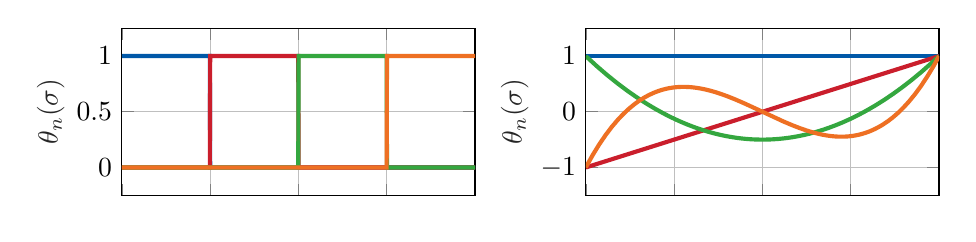
\begin{tikzpicture}

\begin{axis}[%
width=0.37\textwidth,
height=0.175\textwidth,
at={(0\textwidth,0\textwidth)},
scale only axis,
xmin=0,
xmax=1,
xtick={0,0.25,0.5,0.75,1},
xticklabels={{},{},{},{},{}},
ymin=-0.25,
ymax=1.25,
ylabel style={font=\color{white!15!black}},
ylabel={$\theta_n(\sigma)$},
axis background/.style={fill=white},
title style={font=\bfseries},
% title={$(a)$},
xmajorgrids,
ymajorgrids,
ylabel style={yshift=-2.5pt}
]
\addplot [color=mycolor1, line width=1.5pt, forget plot]
  table[row sep=crcr]{%
0	1\\
0.249249249249249	1\\
0.25025025025025	0\\
1	0\\
};
\addplot [color=mycolor2, line width=1.5pt, forget plot]
  table[row sep=crcr]{%
0	0\\
0.249249249249249	0\\
0.25025025025025	1\\
0.499499499499499	1\\
0.500500500500501	0\\
1	0\\
};
\addplot [color=mycolor3, line width=1.5pt, forget plot]
  table[row sep=crcr]{%
0	0\\
0.499499499499499	0\\
0.500500500500501	1\\
0.74974974974975	1\\
0.750750750750751	0\\
1	0\\
};
\addplot [color=mycolor4, line width=1.5pt, forget plot]
  table[row sep=crcr]{%
0	0\\
0.74974974974975	0\\
0.750750750750751	1\\
1	1\\
};
\end{axis}

\begin{axis}[%
width=0.37\textwidth,
height=0.175\textwidth,
at={(0.486\textwidth,0\textwidth)},
scale only axis,
xmin=0,
xmax=1,
xtick={0,0.25,0.5,0.75,1},
xticklabels={{},{},{},{},{}},
ymin=-1.5,
ymax=1.5,
ylabel style={font=\color{white!15!black}},
ylabel={$\theta_n(\sigma)$},
axis background/.style={fill=white},
title style={font=\bfseries},
%title={$(b)$},
xmajorgrids,
ymajorgrids,
ylabel style={yshift=-2.5pt}
]
\addplot [color=mycolor1, line width=1.5pt, forget plot]
  table[row sep=crcr]{%
0	1\\
1	1\\
};
\addplot [color=mycolor2, line width=1.5pt, forget plot]
  table[row sep=crcr]{%
0	-1\\
1	1\\
};
\addplot [color=mycolor3, line width=1.5pt, forget plot]
  table[row sep=crcr]{%
0	1\\
0.0310310310310311	0.819591363134907\\
0.0610610610610611	0.656004352701049\\
0.0900900900900901	0.508156805454103\\
0.118118118118118	0.375002630257885\\
0.145145145145145	0.255531808084361\\
0.171171171171171	0.148770392013635\\
0.196196196196196	0.0537805072339606\\
0.22022022022022	-0.0303396489582677\\
0.243243243243243	-0.10445580715851\\
0.265265265265265	-0.169397625854082\\
0.286286286286286	-0.225958691424157\\
0.307307307307307	-0.277217157097037\\
0.327327327327327	-0.321104888672456\\
0.346346346346346	-0.358343328313298\\
0.364364364364364	-0.389617846074302\\
0.381381381381381	-0.415577739902064\\
0.397397397397397	-0.436836235635034\\
0.413413413413414	-0.455016578139701\\
0.428428428428429	-0.469265060856652\\
0.442442442442442	-0.480122765408051\\
0.456456456456456	-0.488623758894029\\
0.469469469469469	-0.494407320233146\\
0.482482482482482	-0.498158819480141\\
0.495495495495496	-0.499878256635014\\
0.507507507507508	-0.499661823986148\\
0.519519519519519	-0.497713930146363\\
0.532532532532533	-0.493649805962118\\
0.545545545545546	-0.487553619685752\\
0.558558558558559	-0.479425371317263\\
0.572572572572573	-0.468399330261192\\
0.586586586586587	-0.455016578139701\\
0.601601601601602	-0.438062687311937\\
0.617617617617618	-0.416996576155735\\
0.633633633633634	-0.392852311771231\\
0.650650650650651	-0.363826288751214\\
0.668668668668669	-0.329305281257233\\
0.687687687687688	-0.288639991342694\\
0.707707707707708	-0.241145048952857\\
0.727727727727728	-0.188840492143795\\
0.748748748748749	-0.128744359975591\\
0.770770770770771	-0.0600991381772165\\
0.793793793793794	0.0178887596305013\\
0.817817817817818	0.106048991934878\\
0.842842842842843	0.205247289331373\\
0.868868868868869	0.316385454523592\\
0.894894894894895	0.435651868084301\\
0.921921921921922	0.56810864918973\\
0.94994994994995	0.714729744759775\\
0.978978978978979	0.876525173822471\\
1	1\\
};
\addplot [color=mycolor4, line width=1.5pt, forget plot]
  table[row sep=crcr]{%
0	-1\\
0.0190190190190189	-0.782485871940692\\
0.0380380380380381	-0.585849574761409\\
0.0560560560560561	-0.418072891875022\\
0.0740740740740742	-0.267591322461007\\
0.0910910910910911	-0.14071778835241\\
0.107107107107107	-0.0342981766697772\\
0.123123123123123	0.0600275897464979\\
0.138138138138138	0.137912741624562\\
0.153153153153153	0.206008053341874\\
0.167167167167167	0.26108942025359\\
0.18018018018018	0.305205863277448\\
0.193193193193193	0.342823368979655\\
0.205205205205205	0.372007618203764\\
0.216216216216216	0.394270823050955\\
0.227227227227227	0.412405233898399\\
0.237237237237237	0.425443028180901\\
0.246246246246246	0.434472266818126\\
0.255255255255255	0.441030078586554\\
0.264264264264264	0.445204206451941\\
0.272272272272272	0.446984357566612\\
0.28028028028028	0.447012056580584\\
0.288288288288288	0.445348928183114\\
0.297297297297297	0.441533571555485\\
0.306306306306306	0.435743998198344\\
0.316316316316316	0.427102419377978\\
0.327327327327327	0.41505036134801\\
0.339339339339339	0.399043011303921\\
0.352352352352352	0.378569076902044\\
0.367367367367367	0.351233983600084\\
0.383383383383384	0.318131447265587\\
0.401401401401401	0.276624908126279\\
0.422422422422422	0.223395060218871\\
0.447447447447447	0.154754895576799\\
0.481481481481481	0.0554285423969925\\
0.55955955955956	-0.174453117166602\\
0.585585585585586	-0.244218652545899\\
0.606606606606607	-0.295588205146412\\
0.625625625625626	-0.337224912399687\\
0.641641641641642	-0.368091627977139\\
0.656656656656657	-0.393078784510256\\
0.66966966966967	-0.411320689517806\\
0.681681681681682	-0.42510521776274\\
0.692692692692693	-0.434982658462395\\
0.702702702702703	-0.441533571555485\\
0.711711711711712	-0.445348928183114\\
0.720720720720721	-0.447102325115474\\
0.728728728728729	-0.446858939689107\\
0.736736736736737	-0.444855399075886\\
0.744744744744745	-0.441030078586554\\
0.753753753753754	-0.434472266818126\\
0.762762762762763	-0.425443028180901\\
0.771771771771772	-0.413854619709123\\
0.781781781781782	-0.3978703949716\\
0.792792792792793	-0.376369795653945\\
0.803803803803804	-0.350609329511154\\
0.815815815815816	-0.317460398130658\\
0.827827827827828	-0.278843238464521\\
0.840840840840841	-0.230596015489016\\
0.854854854854855	-0.170884130911225\\
0.868868868868869	-0.10280934270289\\
0.883883883883884	-0.020216582116821\\
0.898898898898899	0.0727618041999487\\
0.914914914914915	0.183843708779055\\
0.931931931931932	0.315873496183937\\
0.948948948948949	0.462912686785208\\
0.966966966966967	0.635618141204809\\
0.984984984984985	0.826515637191178\\
1	1\\
};
\end{axis}
\end{tikzpicture}%
  
    % This file was created by matlab2tikz.
%
\definecolor{mycolor1}{rgb}{0.00000,0.34510,0.65882}%
\definecolor{mycolor2}{rgb}{0.79216,0.11765,0.17255}%
\definecolor{mycolor3}{rgb}{0.20392,0.65490,0.24706}%
\definecolor{mycolor4}{rgb}{0.93333,0.43922,0.13725}%
%
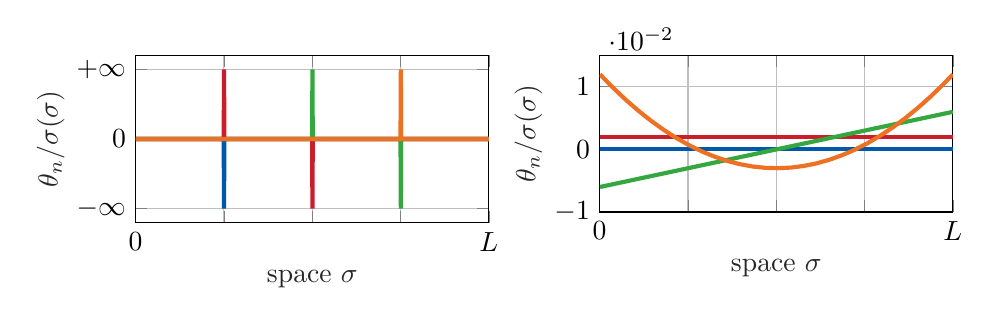
\begin{tikzpicture}

\begin{axis}[%
width=0.37\textwidth,
height=0.175\textwidth,
at={(0\textwidth,0\textwidth)},
scale only axis,
xmin=0,
xmax=1,
xtick={0,0.25,0.5,0.75,1},
xticklabels={{0},{},{},{},{$L$}},
ytick={-1,0,1},
yticklabels={{$-\infty$},0,{$+\infty$}},
xlabel style={font=\color{white!15!black}},
xlabel={space $\sigma$},
ymin=-1.2,
ymax=1.2,
ylabel style={font=\color{white!15!black}},
ylabel={$\p \theta_n/\p \sigma (\sigma)$},
axis background/.style={fill=white},
xmajorgrids,
ymajorgrids,
ylabel style={yshift=-2.5pt}
]
\addplot [color=mycolor1, line width=1.5pt, forget plot]
  table[row sep=crcr]{%
0.00100100100100109	0\\
0.249249249249249	0\\
0.25025025025025	-1\\
0.251251251251251	0\\
1	0\\
};
\addplot [color=mycolor2, line width=1.5pt, forget plot]
  table[row sep=crcr]{%
0.00100100100100109	0\\
0.249249249249249	0\\
0.25025025025025	1\\
0.251251251251251	0\\
0.499499499499499	0\\
0.500500500500501	-1\\
0.501501501501502	0\\
1	0\\
};
\addplot [color=mycolor3, line width=1.5pt, forget plot]
  table[row sep=crcr]{%
0.00100100100100109	0\\
0.499499499499499	0\\
0.500500500500501	1\\
0.501501501501502	0\\
0.74974974974975	0\\
0.750750750750751	-1\\
0.751751751751752	0\\
1	0\\
};
\addplot [color=mycolor4, line width=1.5pt, forget plot]
  table[row sep=crcr]{%
0.00100100100100109	0\\
0.74974974974975	0\\
0.750750750750751	1\\
0.751751751751752	0\\
1	0\\
};
\end{axis}

\begin{axis}[%
width=0.37\textwidth,
height=0.164\textwidth,
at={(0.486\textwidth,0.011\textwidth)},
scale only axis,
xmin=0,
xmax=1,
xtick={0,0.25,0.5,0.75,1},
xticklabels={{0},{},{},{},{$L$}},
xlabel style={font=\color{white!15!black}},
xlabel={space $\sigma$},
ymin=-0.01,
ymax=0.015,
ylabel style={font=\color{white!15!black}},
ylabel={$\p \theta_n/\p \sigma(\sigma)$},
axis background/.style={fill=white},
xmajorgrids,
ymajorgrids,
ylabel style={yshift=-2.5pt}
]
\addplot [color=mycolor1, line width=1.5pt, forget plot]
  table[row sep=crcr]{%
0.00100100100100109	0\\
1	0\\
};
\addplot [color=mycolor2, line width=1.5pt, forget plot]
  table[row sep=crcr]{%
0.00100100100100109	0.00200200200200196\\
1	0.00200200200200196\\
};
\addplot [color=mycolor3, line width=1.5pt, forget plot]
  table[row sep=crcr]{%
0.00100100100100109	-0.00599999398798179\\
1	0.00599999398798179\\
};
\addplot [color=mycolor4, line width=1.5pt, forget plot]
  table[row sep=crcr]{%
0.00100100100100109	0.0119819719820118\\
0.037037037037037	0.00989780573368138\\
0.0730730730730731	0.00796962698002934\\
0.109109109109109	0.00619743572105302\\
0.145145145145145	0.00458123195675597\\
0.181181181181181	0.00312101568713552\\
0.217217217217217	0.00181678691219256\\
0.253253253253253	0.000668545631927309\\
0.289289289289289	-0.000323708153660229\\
0.325325325325325	-0.00115997444457028\\
0.361361361361361	-0.00184025324080306\\
0.397397397397397	-0.0023645445423579\\
0.433433433433434	-0.00273284834923548\\
0.469469469469469	-0.00294516466143557\\
0.505505505505506	-0.00300149347895817\\
0.541541541541542	-0.00290183480180284\\
0.577577577577578	-0.00264618862997024\\
0.613613613613614	-0.00223455496346037\\
0.64964964964965	-0.00166693380227234\\
0.685685685685686	-0.000943325146407048\\
0.721721721721722	-6.37289958642651e-05\\
0.757757757757758	0.000971854649356008\\
0.793793793793794	0.00216342578925377\\
0.82982982982983	0.00351098442382924\\
0.865865865865866	0.00501453055308221\\
0.901901901901902	0.00667406417701244\\
0.937937937937938	0.00848958529562016\\
0.973973973973974	0.0104610939089056\\
1	0.0119819719820118\\
};
\end{axis}
\end{tikzpicture}%
    %\fi
    \vspace{-3mm}
    \caption{Example plot of the Constant-Strain parameterization in Chapter 3 $(a)$, and the new strain parameterization \eqref{eq:C3:chebyshev} using Chebyshev polynomials $(b)$. The ordering of the strain basis is as follows $\{\theta_1,...,\theta_4\} = \{\ldata{Matlab1},\ldata{Matlab2},\ldata{Matlab3},\ldata{Matlab4}\}$. Notice that the discontinuities in the PCC models induce spikes that directly violate the compatibility equation in \eqref{eq:C3:compatibility}.}
    \label{fig:C4:basis_example}
  \end{figure}
  %
\begin{equation}
\theta_n(\sigma) = \dfrac{2}{2^{n}(n-1)!} \dfrac{d^{n-1}}{d\sigma^{n-1}}\left[\left( \dfrac{2\sigma}{L}-1 \right)^2 -1 \right]^{n-1}
\label{eq:C3:chebyshev}
\end{equation}
%
\noindent with $n \in \Z/\{0\}$ the polynomial degree. A comparison between the proposed basis and previous method in Chapter 3 is shown in Figure \ref{fig:C4:basis_example}. Please note now that the inner product between elements of the set of modified Legendre functionals $\{\theta_n\}_{n = 1}^k$ satisfies $\inner{\theta_i}{\theta_j}_{\Xs} := \int_\Xs{\theta_i}{\theta_j} d\sigma = 0$ for $i \neq j$, and $1$ otherwise. An alternative option could be constructing the set of basis functions through the so-called '\textit{snapshot decomposition method}' using FEM-driven data \cite{Astrid2008,Duriez2013,Largilliere2015}.

\begin{rmk}
The idea of joint parameterization by investigating the relation between material and structural topology of the soft robot is explored in Chapter 5.
\end{rmk}

\subsection{Reduced-order curve kinematics}
Given the finite-dimensional truncation in \eqref{eq:trunc_2}, we can now find an expression for the finite-dimensional forward kinematics in terms of the generalized coordinates $\vec{q}$ and its velocities components $\dot{\vec{q}}$.

First, let us regard the configuration of the soft robot $\mat{g} \in \SE{3}$. Recall that the spatial evolution of the curve is described by $\p \mat{g}/\p\sigma = \mat{g} \vec{\xi}^\wedge$, see Eq. \eqref{eq:C3:xi}. Given the initial condition $\mat{g}(0,\cdot) = \mat{g}_0$, an approximation of the continuously deformable soft robot can be obtained by partial integration over the spatial domain:
%
\vspace{-2mm}
\begin{equation}
[\mat{g}]_k(\sigma,\vec{q}) = \mat{g}_0 \exp_{\SE{3}}\left[\int_0^\sigma [\hat{\vec{\xi}}]_k(s,\vec{q}) \; ds \right].
\end{equation}
%
The computation of the mapping $\exp_{\SE{3}}$ is given in Appendix \ref{app:C3:liegroup}. Please note that this nothing more than the reconstruction of the curve by integration of its tangent space along its spatial parameter $\sigma$. Next, lets regard the velocity kinematics $\vec{\eta}(\sigma,t)$ for any point $\sigma$ on the backbone curve. Using the differential property of the adjoint action $\mat{\ad}_{\vec{\xi}} = -\p /\p \sigma [\Ad_{g^{-1}}] \Ad_{g}$ \cite{Murray1994}, we can rewrite the continuous forward kinematics in \eqref{eq:C3:pde_kin} as
%
\begin{equation}
\frac{\p \vec{\eta}}{\p \sigma } = \frac{\p }{\p \sigma }\left(\mat{\Ad}_{\mat{g}^{-1}}\right) \mat{\Ad}_{\mat{g}} \vec{\eta} + \dot{\vec{\xi}}. \label{eq:eta_adg}
\end{equation}
%
Now, given the initial condition $\vec{\eta}(0,t) = \vec{0}_6$ and the approximations $[\vec{\xi}]_k$ and $[\mat{g}]_k$, we can find an approximation to the velocity twist $\vec{\eta}$ by partial integration over space:
%
\begin{equation}
[\vec{\eta}]_k(\sigma,\vec{q},\dot{\vec{q}}) = \Ad_{[\mat{g}]_k}\inv \int_0^\sigma \Ad_{[\mat{g}]_k} \mat{\Theta} \; ds \,\dot{\vec{q}} := [\mat{J}]_k\, \dot{\vec{q}}, \label{eq:C3:eta_analytic}
\end{equation}
%
which naturally gives rise to the geometric Jacobian $[\mat{J}]_k \in \R^{6\times 6k}$. The geometric Jacobian plays an important role in obtaining the Lagrangian form of the reduced-order dynamic model. Finally, to express the acceleration twist, we take the time-derivative of \eqref{eq:C3:eta_analytic} leading to
%
\begin{align}{}
[\dot{\vec{\eta}}]_k & = [\mat{J}]_k\ddot{\vec{q}} + \dot{[\mat{J}]}_k\dot{\vec{q}}, \notag \\
& = [\mat{J}]_k\ddot{\vec{q}} + \Ad_{[\mat{g}]_k}\inv \int_0^\sigma \Ad_{[\mat{g}]_k} \ad_{[\vec{\eta}]_k} \mat{\Theta} \; ds \,\dot{q} \label{eq:C3:deta_analytic},
\end{align}
%
which gives rise to the analytic expression of the time-derivative of the geometric Jacobian $\dot{[\mat{J}]}_k$ (see Appendix \ref{app:C3:jacobian} for the derivation).

\subsection{Reduced-order curve dynamics using Newton-Euler}
Here, we detail the dynamics of the Cosserat beam. A majority of the dynamic framework presented here is adopted from Boyer et al. (2021, \cite{Boyer2021}); yet we introduce some modification to allow a pH-structure. First, let us consider an infinitesimal slice of continuum body that is perpendicular to the backbone curve. The kinetic momenta of this infinitesimal slice is then given by $\vec{\mu}(\sigma,t) := \MT \vec{\eta}(\sigma,t)$ in which $\MT \in \cose{3} \times \seg{3} \cong \R^{6\times 6}$ denotes the symmetric inertia tensor.
%
\begin{rmk}
For some soft robots, the inertia tensor $\MT$ may have an explicit dependency on space or time (or both). Nevertheless, for sake of simplicity, we limit ourselves to a diagonal invariant inertia tensor:
%
\begin{equation*}
\MT(\sigma,t) \cong \MT = \begin{pmatrix} \rho_0 \ten{J}  & \vec{0}_{3\times3}  \\[0.35em]
  \vec{0}_{3\times3} & \rho_0\, A\mat{I}_3 \end{pmatrix} \succ 0,
\end{equation*}
%
in which the (cross-sectional average) density is $\rho_0 > 0$, the cross-sectional area of the soft robot by $A>0$, and the second moment of area $\mat{\mathcal{J}} \in \coso{3} \times \sog{3} \cong \R^{3\times 3}$.
\end{rmk}
%
\noindent Using the expression of the kinetic momenta $\muB(\sigma,t)$ of the infinitesimal rigid body in free-motion, we can write the equation of motion for a particular slice at $\sigma$ using the Newton-Euler equations:
%
\begin{equation}
\frac{\p }{\p t} (\Ad_{\gB}^{-\top} \vec{\mu}) = \Ad_{g}^{-\top}\ten{F},\label{eq:C3:newton_euler}
\end{equation}
%
where again $\Ad_{(\cdot)}$ stands for the adjoint action, and $\ten{F} = \ten{F}_c  + \ten{F}_u - \ten{F}\grav - \ten{F}\elastic$ the resultant wrench that is composed of the constraint wrench $\ten{F}_c$, the input wrench $\ten{F}_u$, and the potential wrenches due to gravity and visco-elasticity, $\ten{F}\grav$ and $\ten{F}\elastic$, respectively. Further evaluation of \eqref{eq:C3:newton_euler} leads to
%
\begin{equation}
\MT\dot{\vec{\eta}} - \ad_{\vec{\eta}}^\top \MT \vec{\eta} = \ten{F},
\label{eq:C3:newton-euler-2}
\end{equation}
%
where we used the fact that $\dot{\Ad}_{\vec{g}} \inv = -\ad_{\vec{\eta}} {\Ad}_{\vec{g} \inv}$. Before continuing, we introduce a slight modification to the relation above. Using the fact that $\ad_{\vec{\eta}} \vec{\eta} = \vec{0}_6$, we can introduce the vector
$\ten{M} \ad_{\vec{\eta}} \vec{\eta}$ to \eqref{eq:C3:newton-euler-2} without affecting the dynamics. The importance of this modification originates from the preservation of passivity in the Lagrangian model, which is an important property in stability theorems for robotics. By substitution of the null vector, the equation of motion becomes
%
\begin{equation}
  \MT \dot{\vec{\eta}} + \left(\MT \ad_{\vec{\eta}}  - \ad_{\vec{\eta}} ^\top \MT \right) \vec{\eta} = \FT,
  \label{eq:C3:newton-euler-3}
\end{equation}
%
which is nothing more than the Newton-Euler equation for rigid-body motion on $\R^3$. To introduce the (reduced-order) Cosserat kinematics and make the expression symmetric, we substitute \eqref{eq:C3:eta_analytic} and \eqref{eq:C3:deta_analytic} into \eqref{eq:C3:newton-euler-3} and pre-multiply by $[\JB]_k^\top$:
%
\begin{multline}
  [\vec{J}]_k^\top \left( \MT [\mat{J}]_k \ddot{\vec{q}} + \MT [\dJB]_k\dot{\vec{q}} + \CT_{[\vec{\eta}]_k }\dot{\vec{q}}\right) = [\mat{J}]_k^\top \left(\FT_u - \FT\grav - \FT\elastic \right),
  \label{eq:C3:projected_NE_jacobian}
\end{multline}
%
where $\CT_{(\cdot)} = -\CT_{(\cdot)} ^\top :=  \MT \ad_{(\cdot)}  - \ad_{(\cdot)} ^\top \MT$ is a skew-symmetric matrix. It is important to note that by pre-multiplication of the transpose Jacobian, we have eliminated the constraint wrenches, \ie, $[\JB]_k^\top \FT_c = \vec{0}_n$ \cite{Murray1994}. Finally, the finite-dimensional dynamics of the deformable soft robot is found by spatial integration of \eqref{eq:C3:projected_NE_jacobian} over the material domain $\Xs$. The overall dynamics can be written in familiar Euler-Lagrangian (EL) form as follows
%
\begin{equation}
  \mat{M}(\vec{q})\ddot{\vec{q}} + \mat{C}(\vec{q},\dot{\vec{q}})\dot{\vec{q}} + \vec{f}\!\grav(\vec{q}) + \vec{f}\!\elastic(\vec{q},\dot{\vec{q}}) = \vec{\tau}(\vec{q},\uB)
  \label{eq:C3:dyn_model_lag}
\end{equation}
%
with the system matrices:
%
\begin{align}
 \MB(\q) & = \int_\Xs [\mat{J}]_k^\top \ten{M} [\mat{J}]_k \; d \sigma, \label{eq:C3:lag_M} \\
 \mat{C}(\q,\dq) & = \int_\Xs [\JB]_k^\top \!\left(\ten{M} [\dJB]_k + \ten{C}_{{[\vec{\eta}]}_k}[\mat{J}]_k \right) \; d \sigma, \label{eq:C3:lag_C} \\
\vec{f}\!\grav(\q) & = \int_\Xs [\JB]_k^\top \ten{F}\!\grav \; d \sigma, \\
\vec{f}\!\elastic(\q,\dq) & = \int_\Xs [\JB]_k^\top \ten{F}\!\elastic \; d \sigma := \mat{K}\vec{q} + \mat{D}\dot{\vec{q}},
\label{eq:C3:lag_G} \\
\vec{\tau}(\q,\uB) & = \int_\Xs [\mat{J}]_k^\top \ten{F}_u \; d\sigma := \mat{G} \vec{u}, \label{eq:C3:lag_tau}
\end{align}
%
\noindent where $\mat{M}$ is the generalized inertia matrix, $\mat{C}$ the  centripetal-Coriolis matrix, $\fB\!\grav$ a vector of generalized potential forces with $\ten{F}\!\grav = -\Ad_{[\gB]_k}^\top \ten{M} \vec{a}_g$ the external wrench acting on the body due to gravitational acceleration $\vec{a}_g$, and $\ten{F}_e$ a vector of visco-elastic forces imposed by the stiffness matrix $\mat{K} \succ 0$ and damping matrix $\vec{D} \succ 0$. Following the procedures in finite elements and assuming linear visco-elasticity, the stiffness matrix and damping matrix are computed through spatial integration:
%
\begin{align}
\mat{K} = \int_\Xs \mat{\Theta}^\top \!\mat{\mathcal{K}}\, \mat{\Theta} \; d\sigma, \label{eq:C3:stiff_mat}\\
\mat{D} = \int_\Xs \mat{\Theta}^\top \!\mat{\mathcal{D}}\, \mat{\Theta} \; d\sigma, \label{eq:C3:damp_mat}
\end{align}
%
where $\mat{\mathcal{K}} \in \cose{3} \times \seg{3}$ and $\mat{\mathcal{D}} \in  \cose{3} \times \seg{3}$ are the stiffness and damping tensor, respectively. The vector $\vec{Gu}$ represents the distributed forces and torques generated by various kinds of the internal actuators (\eg, tendons or pneumatics). Again, system of matrices can then be efficiently recovered using a Matrix-Differential solver proposed in Chapter 3. If $\rank(\GB) < \dim(\q)$, a system is said to be under-actuated. Within the context of soft robotics, whose infinite-dimensional configuration space cannot be matched by a finite number of actuators, these systems are often intrinsically under-actuated. 

\begin{lem}
  \label{lem:C3:1}
  The inertia matrix $\mat{M}(\vec{q})$ is a symmetric, positive definite, symmetric. and is uniformly bounded such that there exists positive constants $\lambda^{-} \le \lambda^{+}$ such that  $\lambda^{-} \mat{I}_{n} \preceq \mat{M}(\vec{q}) \preceq \lambda^{+} \mat{I}_{n} < \infty$.
\end{lem}

\begin{proof}
Proof can be found in Spong et al. (2006, \citep{Spong2006}).
\end{proof}

\begin{lem}
\label{lem:C3:passive}
Given the inertia matrix $\mat{M}(\vec{q})$ and the Coriolis matrix
$\mat{C}(\vec{q},\dot{\vec{q}})$ as described by \eqref{eq:C3:lag_M} and \eqref{eq:C3:lag_C}, respectively, it can be shown that the matrix $\dot{\mat{M}} - 2\mat{C}$ is skew-symmetric.
\end{lem}

\begin{proof}
To show $\dot{\mat{M}} - 2\mat{C}$ is skew-symmetric, we start by computing the time-derivative of the inertia matrix. For sake of clarity, lets abbreviate the Jacobians matrices $[\mat{J}]_k = \mat{J}$ and $[\dJB]_k = \dJB$. Through chain differentiation, we find
%
\begin{equation}
\dot{\mat{M}} = \int_\Xs \dJB^\top \ten{M} \mat{J} + \mat{J}^\top \ten{M} \dJB\; d \sigma,
\end{equation}
%
Then, calculating $\dot{\mat{M}} - 2\mat{C}$ leads to
%
\begin{align}
\dot{\mat{M}} - 2\mat{C} & = \int_\Xs \dJB^\top \ten{M} \mat{J} - \mat{J}^\top \ten{M} \dJB - 2\mat{J}^\top \!\ten{C} \, \mat{J} \; d\sigma.
\end{align}
%
Since the matrix $\mat{J}^\top \ten{C} \mat{J}$ is skew-symmetric, the remainder of the proof is to show that the matrix $\mat{S} = \dJB^\top \ten{M} \mat{J} - \mat{J}^\top \ten{M} \dJB$ also satisfies skew-symmetry. Since the inertia tensor is symmetric $\ten{M} = \ten{M}^\top
$, we can easily show this holds true:
%
\begin{align}
\mat{S} & = \dJB^\top \MT^\top \mat{J} - \mat{J}^\top \MT^\top \dJB, \notag \\
 & = -\left(\dJB^\top \ten{M}^\top \mat{J} - \mat{J}^\top \ten{M} \dJB \right)^\top = -\mat{S}^\top.
\end{align}
%
Therefore, the matrix $\dot{\mat{M}(\vec{q})} - 2\mat{C}(\vec{q},\dot{\vec{q}})$ is skew-symmetric for all $\vec{q},\dot{\vec{q}} \in \R^n$
\end{proof}

In literature, Lemma \ref{lem:C3:passive} is often referred to as the passivity condition \cite{Spong2006,Ortega1998,Murray1994}. It implies that, in the absence of external dissipation, the total energy of the system (\ie, the Hamiltonian) is conserved. It is also worth mentioning that this condition does not necessarily hold true for all cases, only for particular computations of the Coriolis matrix $\mat{C}(\vec{q},\vec{\dot{q}})$ (\eg, through the Christoffel symbols).

\subsection{Port-Hamiltonian formulation}
In this section, the Lagrangian model in \eqref{eq:C3:dyn_model_lag} is rewritten in port-Hamiltonian form. To this end, we define the generalized momenta $\vec{p} := \mat{M} \dot{\vec{q}}$. Then, the (reduced-order) Hamiltonian is given by
$\mathcal{H}(\vec{q},\vec{p}) := \Kf(\vec{q},\vec{p}) + \Uf(\vec{q})$ with $\Kf = \frac{1}{2} \vec{p}^\top \mat{M}\inv \vec{p}$ and $\Uf(\vec{q})$ the kinetic and potential energy, respectively.

Given the system's Hamiltonian $\mathcal{H}$, it can be shown that generalized velocities can be written in terms of partial derivatives of the Hamiltonian function
%
\begin{equation}
\dot{\vec{q}} = \nabla_{\vec{p}} \Hm \quad \Longrightarrow  \quad \nabla_{\vec{p}} \Hm := \left(\frac{\p \Hm}{\p \pB} \right)^\top= \mat{M}\inv \vec{p}.
\label{eq:C3:state_diff}
\end{equation}
%
where we denote $\nabla_{\xB}(\cdot) := \p (\cdot)^\top/\p \xB$ as the gradient w.r.t. a vector field $\xB$. Note that $\mat{M}^{-1}$ is always exists due to the positive definiteness condition in Lemma \ref{lem:C3:1}. Similarly, we seek a differential description that relates the time evolution of $\vec{p}$ to a state-derivative of the Hamiltonian function. Applying the chain rule of differentiation to the generalized momenta:
%
\begin{align}
\dot{\vec{p}} & = \dot{\mat{M}}\dot{\vec{q}} + \mat{M}\ddot{\vec{q}},\notag \\
& = \left(\dot{\mat{M}} - \mat{C} - \mat{D} \right) \mat{M}\inv \vec{p} - \vec{Kq} - \vec{f}\!\grav + \vec{Gu}
\label{eq:C3:momenta_diff1},
\end{align}
%
Taking the partial derivative of the Hamiltonian $\Hm$ w.r.t. the generalized coordinates $\vec{q}$, we find
 %
\begin{align}
\nabla_{\vec{q}} \Hm & = \frac{1}{2} \,\nabla_{\!\q} \left[ \dot{\vec{q}}^\top \mat{M}(\vec{q}) \dot{\vec{q}} \right] + \nabla_{\!\vec{q}}\, \mathcal{U}.
\label{eq:C3:ham_momenta_diff}
\end{align}
%
To relate \eqref{eq:C3:momenta_diff1} and \eqref{eq:C3:ham_momenta_diff}, we explores some structural properties in the Lagrangian model. To be more specific, we exploit the skew-symmetry condition as detailed in Lemma \ref{lem:C3:passive}. According to the Spong et al. (2006, \cite{Spong2006}), if the matrix $\dot{\mat{M}} - 2\mat{C}$ satisfies the passivity condition in Lemma \ref{lem:C3:passive}, it can be shown that
%
\begin{equation}
\left( \dot{\mat{M}} - 2\mat{C} \right) \dot{\vec{q}} =  -\nabla_{\vec{q}} \left[ \dot{\vec{q}}^\top \mat{M}(\vec{q}) \dot{\vec{q}} \right] - \dot{\mat{M}}\dot{\vec{q}}. \label{eq:C3:skew_mat_equal}
\end{equation}
%
Finally, by combining \eqref{eq:C3:state_diff}, \eqref{eq:C3:momenta_diff1}, \eqref{eq:C3:ham_momenta_diff}, and \eqref{eq:C3:skew_mat_equal}, we can show that the Lagrangian model in \eqref{eq:C3:dyn_model_lag} can be equivalently rewritten as a standard port-Hamiltonian (pH) system:
\begin{align}
\Sigma_{\textrm{beam}}: 
\begin{cases}
\dot{\vec{q}} \;=\; \nabla_{\vec{p}} \Hm, \\[0.25em]
\dot{\vec{p}} \;=\; -\nabla_{\vec{q}} \Hm - \mat{D}\nabla_{\vec{p}} \Hm + \vec{Gu}.
\end{cases}
\label{eq:C3:model_ph}
\end{align}
%
The advantage of the port-Hamiltonian system $\Sigma_\textrm{beam}$ over the standard EL structure in \eqref{eq:C3:dyn_model_lag}, and as also seen in Chapter 3, is the general applicability to different physical domains and the common formalism with energy-based control, which we will explore further in the next section. By collocating the state variable into a state vector $\x = (\q^\top, \pB^\top)^\top$, we may write the system into an equivalent form: $\dx = \left(\JT - \RT \right)\grad{\x}\!\Hm(\x) + \BT(\x)\uB$, where $\JT = -\JT^\top$ a skew-symmetric matrix, $\RT \succeq 0$ a positive semi-definite dissipation matrix. 

\section{Energy-based controller for tasks on $\SE{3}$} \label{sec:chap3_control}
%!TEX root = ../../thesis.tex
Given the previous reduced-order dynamic model, our objective here is to find a controller $\vec{u}$ that ensures $\lim_{t\to\infty} \mat{g}(L,t) = \mat{g}_d$ in which $\mat{g}_d \in \SE{3}$ denotes the desired configuration of the end-effector. To achieve the control objective, the main idea is to reshape the potential energy function of the reduced-order finite-dimensional system using a standard energy-shaping techniques, common to standard port-controlled Hamiltonian models \cite{Schaft2004,Ortega2002}.

%\subsection{Setpoint regulation on $\SE{3}$}
We adopted an energy-based control strategy akin to the works of Franco et al. (2020, \cite{Franco2020}), Ortega et al. (1988, \cite{Ortega1998,Ortega2002}) and Schaft (2004, \cite{Schaft2004}). Following the energy-shaping strategy, the model-based nonlinear controller becomes
%
\begin{equation}
\vec{u} = \vec{G}\ginv \left( \nabla_{\vec{q}}\Hm - \nabla_{\vec{q}}\Hm_d \right),
\label{eq:C3:control}
\end{equation}
%
where $\mat{G}\ginv = \bigl(\mat{G}^\top \mat{G}\bigr)\inv \mat{G}^\top$ is the generalized inverse of the actuation map $\mat{G}$, and the desired Hamiltonian in closed loop
$\Hm_d = \frac{1}{2} \vec{p}^\top \mat{M}\inv \vec{p} + \Uf_d$ that satisfies $\textrm{argmin}_{\mat{g}_L} \Uf_d = \mat{g}_d$ with $\mat{g}_L = \mat{g}(L,\cdot)$ the pose of the end-effector. Note that we purposefully omitted any damping injection as the system's intrinsic visco-elastic damping is deemed sufficiently large to guarantee stability. Following the concept of a kinematic feedback controller \cite{Bullo1995,Boyer2021} that artificially mimic an elastic element between the end-effector and the desired configuration in $\SE{3}$, we have choose the gradient of the desired potential energy as
%
\begin{equation}
\grad{\q}\,\Uf_{d}= \lambda_1 \mat{J}^\top\bigl(\mat{J J}^\top + \lambda_2 \mat{I} \bigr)\inv \ten{F}_u,
\label{eq:C3:jacob_damped}
\end{equation}
%
where $\lambda_1 >0$ is a proportional gain, $\lambda_2 > 0$ a controller gain related to the artificial damping of the pseudo-inverse, $\ten{F}_u = k_p T_{SE(3)}(\mat{\mathcal{E}})\mat{\mathcal{E}}$ an artificial control wrench with positive definite stiffness matrix $k_p$, $\mat{\mathcal{E}} = \log_{\SE{3}} ([\mat{g}_L]_k \inv \mat{g}_d)$ where $\log_{\SE{3}}(\cdot)
$ and $T_{\SE{3}}(\cdot)$ denote the logarithmic map (see Appendix \ref{app:C3:liegroup}) and the tangent-space map, respectively. We refer the reader to Sonneville et al. (2014, \cite{Sonneville2014}) for the numerical computations of the tangent map on $\SE{3}$. The vector $\vec{\mathcal{E}}$ may be regarded as the geometric error between the homogeneous transformations $\mat{g}_d$ and $\mat{g}_L$ such that if $\mat{g}_d = \mat{g}_L$ will simply yield $\lVert \vec{\mathcal{E}} \rVert_2 = 0$. Furthermore, the controller gains $\lambda_1$ and $\lambda_2$ can be tuned accordingly to tweak the desired transient behavior of the closed-loop system, similar to a classical PD controller.

%\newpage
\section{Simulation studies of bio-inspired robots} \label{sec:chap3_result}
%!TEX root = ../../thesis.tex
In this section, we detail the numerical simulations of the port-Hamiltonian model in \eqref{eq:C3:model_ph} together with the energy-shaping controller in \eqref{eq:C3:control}. For all numerical simulations, we consider a truncation degree of the ROM model is $k = 8$.

Due to the partial differential nature, we have to employ a nested ODE routine to recover the trajectories for $\vec{q}$ and $\vec{p}$. First, we employ an implicit trapezoidal solver with a fixed stepsize of $dt = 30 $ ms to solve \eqref{eq:C3:model_ph}. At each time increment, we have to evaluate the dynamic matrices \eqref{eq:C3:lag_M}-\eqref{eq:C3:lag_tau}. To efficiently compute these dynamic entities, we solve the spatial integration problem over the material domain $\Xs$ by using a second-order Runge-Kutta solver. The stepsize for the spatial solver is $d\sigma = 5$ mm. All simulation examples and underlying source code are provided publicly on the \sorotoki toolkit
\cite{Caasenbrood2020}. Here, the numerical integrations of the system matrices \eqref{eq:C3:lag_M}, \eqref{eq:C3:lag_C}, \eqref{eq:C3:lag_G} and \eqref{eq:C3:lag_tau} are performed using a so-called Matrix-Differential solver (see \cite{Caasenbrood2022}). The simulations are performed on a modern machine (Ryzen 7-5800H, 3.2GHz).

For the soft robotic simulations, we have chosen a linear isotropic Hookean material with shear constraints. %Although hyper-elastic material models are possible, e.g, Neo-Hookean or Yeoh, it is considered out of the scope of this work (see \cite{Kim2018,Renaud2011}). 
Given these material properties, the inertia tensor and the stiffness tensor become diagonal matrices:
%
\begin{align*}
\mat{\mathcal{M}} & = \blkdiag{ \rho_0 \mat{\mathcal{J}},\, \rho_0 A \mat{I}_3}; \\[0.45em]
\mat{\mathcal{K}} & = \blkdiag{\mu_1 \mat{\mathcal{J}},\, E A,\, \mu_2  A,\,\mu_2  A},
\end{align*}
%
where the (average) cross-sectional is $A = \pi r^2$ for a disc radius $r$, and $\mat{\mathcal{J}}$ the second moment of area. The damping tensor chosen as $\mat{\mathcal{D}} = \zeta \mat{\mathcal{K}}$ with damping coefficient $\zeta$. The visco-elastic matrices are precomputed using \eqref{eq:C3:stiff_mat} and \eqref{eq:C3:damp_mat}.

\subsection{Soft robot manipulator inspired by octopus' tentacle}
In the first study-case, we consider a soft robotic arm that is loosely inspired by the tentacles of an octopus. To introduce the under-actuation typically present in soft robotics, we have chosen an actuation matrix $\mat{G} = \blkdiag{\mat{I}_5, \mat{O}_3}$ such that only the first five modes are actively controllable. The system  properties can shown in Table \ref{tab:C3:parameters1}.
%
\begin{table}[t]
  \vspace{-0.25cm}
  \caption{Parameters setting for the numerical solver, the soft manipulator, and the energy-based controller.}\label{tab:C3:parameters1} \centering
  \begin{tabular}{l|c|c|l}
    Parameter description & Symbol & Value & Unit \\
    \midrule
    Finite horizon time & $T $ & $10$ & s \\
    Intrinsic length & $L $ & $ 120$ & mm \\
    Cross-section radius & $r $ & $ 8.25$ & $\text{mm}$ \\
    Uniform density & $\rho_0 $ & $ 1250$ & $\text{kg}\text{m}^{-3}$ \\
    %Gravitational acceleration & $a_{g} $ & $ 9.81$ & $\text{m}\text{s}^{-2}$ \\
    Young's modulus & $E $ & $ 25$ & $\text{MPa}$ \\
    Shear modulus & $\mu_1 $ & $ 10 $ & $\text{MPa}$ \\
    Constraint modulus & $\mu_2 $ & $ 15 $ & $\text{GPa}$ \\
    Rayleigh coefficient & $\zeta $ & $ 0.40 $ & - \\
    \bottomrule
  \end{tabular}
  \vspace{-3mm}
  \end{table}
%
The soft robot is subjected to the energy-based controller in \eqref{eq:C3:control}, where the control gains are tuned to produce a smooth transient: $\lambda_1 = 0.01$ and $\lambda_2 = 0.001$. The artificial spring stiffness is chosen as $\mat{k}_p = \blkdiag{0.01\cdot \mat{I}_3, \mat{I}_3}$. Lastly, the desired configuration of the end-effector is chosen as follows:
%
\begin{equation*}
\mat{g}_d = \begin{pmatrix} \mat{I}_3 & \mat{r}_d \\ \vec{0}_3^\top & 1 \end{pmatrix} \quad \text{with} \quad \mat{r}_d = \begin{pmatrix}  0.04 \\ 0.00 \\ -0.01  \end{pmatrix}.
\end{equation*}
%
The numerical results of the closed-loop system are shown in Figure \ref{fig:octarm1} and \ref{fig:octarm1_states}. It is worth mentioning that these simulation run at $\pm120$ \si{\hertz} real-time.$^{1}$ \blankfootnote{$^{1}$Real-time bandwidth is determined by the ratio between finite horizon and CPU's computation time, \ie, $f \approx T/T_{\textrm{sim}}$,which is affected most by spatial stepsize due to explicit integration.} 

Figure \ref{fig:octarm1} shows the evolution of the continuous deformation along the soft robotic body, whereas Figure \ref{fig:octarm1_states} shows the modal coefficients $\vec{q}(t)$ and generalized momenta $\vec{p}(t)$. As can be seen, the end-effector of the soft robot manipulator slowly converges to the desired set-point $\mat{g}_d \in \SE{3}$. Although the control gains could be increased to promote a faster transient, it was observed that high gains lead to undesired (propagating) oscillations of the flexible structure. A possible solution might be to introduce negative damping to the controller Hamiltonian $\Hm_d$, to overcome the soft robot's structural damping.

For the second simulation run, we modified the control gains to highlight an interesting property of the proposed controller. To be more specific, we increase the controller gains to $\lambda_1 = \lambda_2 = 0.1$. The numerical results for the increased controller gains are shown in Figure \ref{fig:octarm2} and Figure \ref{fig:octarm2_states}. Although the control goal and the initial conditions are chosen identical, the soft robot converges to a different configuration -- albeit, a shape with less '\textit{complexity}'. The cause of less complicated bending patterns has two origins. First, increasing the control gains also artificially impacts the structural stiffness of the soft robot, resulting in soft robot with a higher perceived stiffness. Second, by increasing the stabilizing term $\lambda_2$ in the damped Jacobian inverse \eqref{eq:C3:jacob_damped}, more weight is given towards finding a solution that also minimizes the joint angles $\lVert \vec{q} \rVert_2 $. As intrinsically, more energy is spent to excite higher-order modes in the basis $\{\theta_n\}_{n=1}^k$, the energy-based controller will thus find a minimizer that accounts for the ordering of the shape basis, penalizing higher-order modes. This result indicates that the proposed controller can be effectively tuned alter the structural compliance of the soft robot; and thus could be implemented carefully to preserve '\textit{softness}'. 

\afterpage{
  \vfill
  \begin{figure*}[!t]
    \centering
    \vspace{-12mm}
    % This file was created by matlab2tikz.
%
\begin{tikzpicture}

\begin{axis}[%
width=0.783\textwidth,
height=0.541\textwidth,
at={(0.121\textwidth,0\textwidth)},
scale only axis,
xmin=0,
xmax=1,
ymin=0,
ymax=1,
axis line style={draw=none},
ticks=none,
axis x line*=bottom,
axis y line*=left,
colorbar style={width=6,xshift=-7.5pt}
]
\end{axis}

\begin{axis}[%
width=0.31\textwidth,
height=0.149\textwidth,
at={(0\textwidth,0.413\textwidth)},
scale only axis,
axis on top,
xmin=0.5,
xmax=1024.5,
tick align=outside,
y dir=reverse,
ymin=0.5,
ymax=512.5,
axis line style={draw=none},
ticks=none,
colorbar style={width=6,xshift=-7.5pt}
]
\addplot [forget plot] graphics [xmin=0.5, xmax=1024.5, ymin=0.5, ymax=512.5] {fig_C3_3D_srmsoft-1.png};
\end{axis}

\begin{axis}[%
width=0.31\textwidth,
height=0.149\textwidth,
at={(0.34\textwidth,0.413\textwidth)},
scale only axis,
axis on top,
xmin=0.5,
xmax=1024.5,
tick align=outside,
y dir=reverse,
ymin=0.5,
ymax=512.5,
axis line style={draw=none},
ticks=none,
colorbar style={width=6,xshift=-7.5pt}
]
\addplot [forget plot] graphics [xmin=0.5, xmax=1024.5, ymin=0.5, ymax=512.5] {fig_C3_3D_srmsoft-2.png};
\end{axis}

\begin{axis}[%
width=0.31\textwidth,
height=0.149\textwidth,
at={(0.68\textwidth,0.413\textwidth)},
scale only axis,
axis on top,
xmin=0.5,
xmax=1024.5,
tick align=outside,
y dir=reverse,
ymin=0.5,
ymax=512.5,
axis line style={draw=none},
ticks=none,
colorbar style={width=6,xshift=-7.5pt}
]
\addplot [forget plot] graphics [xmin=0.5, xmax=1024.5, ymin=0.5, ymax=512.5] {fig_C3_3D_srmsoft-3.png};
\end{axis}

\begin{axis}[%
width=0.31\textwidth,
height=0.149\textwidth,
at={(0\textwidth,0.214\textwidth)},
scale only axis,
axis on top,
xmin=0.5,
xmax=1024.5,
tick align=outside,
y dir=reverse,
ymin=0.5,
ymax=512.5,
axis line style={draw=none},
ticks=none,
colorbar style={width=6,xshift=-7.5pt}
]
\addplot [forget plot] graphics [xmin=0.5, xmax=1024.5, ymin=0.5, ymax=512.5] {fig_C3_3D_srmsoft-4.png};
\end{axis}

\begin{axis}[%
width=0.31\textwidth,
height=0.149\textwidth,
at={(0.34\textwidth,0.214\textwidth)},
scale only axis,
axis on top,
xmin=0.5,
xmax=1024.5,
tick align=outside,
y dir=reverse,
ymin=0.5,
ymax=512.5,
axis line style={draw=none},
ticks=none,
colorbar style={width=6,xshift=-7.5pt}
]
\addplot [forget plot] graphics [xmin=0.5, xmax=1024.5, ymin=0.5, ymax=512.5] {fig_C3_3D_srmsoft-5.png};
\end{axis}

\begin{axis}[%
width=0.31\textwidth,
height=0.149\textwidth,
at={(0.68\textwidth,0.214\textwidth)},
scale only axis,
axis on top,
xmin=0.5,
xmax=1024.5,
tick align=outside,
y dir=reverse,
ymin=0.5,
ymax=512.5,
axis line style={draw=none},
ticks=none,
colorbar style={width=6,xshift=-7.5pt}
]
\addplot [forget plot] graphics [xmin=0.5, xmax=1024.5, ymin=0.5, ymax=512.5] {fig_C3_3D_srmsoft-6.png};
\end{axis}

\begin{axis}[%
width=0.31\textwidth,
height=0.149\textwidth,
at={(0\textwidth,0.015\textwidth)},
scale only axis,
axis on top,
xmin=0.5,
xmax=1024.5,
tick align=outside,
y dir=reverse,
ymin=0.5,
ymax=512.5,
axis line style={draw=none},
ticks=none,
colorbar style={width=6,xshift=-7.5pt}
]
\addplot [forget plot] graphics [xmin=0.5, xmax=1024.5, ymin=0.5, ymax=512.5] {fig_C3_3D_srmsoft-7.png};
\end{axis}

\begin{axis}[%
width=0.31\textwidth,
height=0.149\textwidth,
at={(0.34\textwidth,0.015\textwidth)},
scale only axis,
axis on top,
xmin=0.5,
xmax=1024.5,
tick align=outside,
y dir=reverse,
ymin=0.5,
ymax=512.5,
axis line style={draw=none},
ticks=none,
colorbar style={width=6,xshift=-7.5pt}
]
\addplot [forget plot] graphics [xmin=0.5, xmax=1024.5, ymin=0.5, ymax=512.5] {fig_C3_3D_srmsoft-8.png};
\end{axis}

\begin{axis}[%
width=0.31\textwidth,
height=0.149\textwidth,
at={(0.68\textwidth,0.015\textwidth)},
scale only axis,
axis on top,
xmin=0.5,
xmax=1024.5,
tick align=outside,
y dir=reverse,
ymin=0.5,
ymax=512.5,
axis line style={draw=none},
ticks=none,
colorbar style={width=6,xshift=-7.5pt}
]
\addplot [forget plot] graphics [xmin=0.5, xmax=1024.5, ymin=0.5, ymax=512.5] {fig_C3_3D_srmsoft-9.png};
\end{axis}
\end{tikzpicture}%
    \vspace{-1mm}
    \caption{Three-dimensional evolution of the soft robot manipulators, slowly converging to the desired set-point $g_d \in \SE{3}$ (indicated by the pink ball). Please observe the morphology that arises which can be related to the motion of an octopus. }
    \label{fig:octarm1}
  \end{figure*}
  \vspace{2mm}
  \begin{figure}[!t]
    \centering
    \vspace{-20mm}
    % This file was created by matlab2tikz.
%
\definecolor{mycolor1}{rgb}{0.00000,0.34510,0.65882}%
\definecolor{mycolor2}{rgb}{0.79216,0.11765,0.17255}%
\definecolor{mycolor3}{rgb}{0.20392,0.65490,0.24706}%
\definecolor{mycolor4}{rgb}{0.93333,0.43922,0.13725}%
\definecolor{mycolor5}{rgb}{0.49412,0.14510,0.51373}%
\definecolor{mycolor6}{rgb}{0.97647,0.67059,0.08235}%
\definecolor{mycolor7}{rgb}{0.24314,0.18039,0.52549}%
\definecolor{mycolor8}{rgb}{0.71373,0.81961,0.14118}%
%
\begin{tikzpicture}

\begin{axis}[%
width=0.37\textwidth,
height=0.3\textwidth,
at={(0\textwidth,0\textwidth)},
scale only axis,
xmin=0,
xmax=6,
xlabel style={font=\color{white!15!black}},
xlabel={time (s)},
ymin=-0.08,
ymax=0.05,
ylabel style={font=\color{white!15!black}},
ylabel={$\vec{q}(t)$},
axis background/.style={fill=white},
xmajorgrids,
ymajorgrids,
ylabel style={yshift=-9.5pt}
]
\addplot [color=mycolor1, line width=1.5pt, forget plot]
  table[row sep=crcr]{%
0	0.00100000000000033\\
0.0999999999999996	0.000732535763058095\\
0.2	0.000833074040049731\\
0.983333333333333	0.00293974513825557\\
1.88333333333333	0.00385980750118531\\
3.56666666666667	0.00456401284455943\\
5.98333333333333	0.00467530988040199\\
};
\addplot [color=mycolor2, line width=1.5pt, forget plot]
  table[row sep=crcr]{%
0	0.00100000000000033\\
0.0666666666666664	0.000815426863866264\\
0.166666666666667	2.29049321793795e-05\\
0.533333333333333	-0.000711551703824753\\
1.08333333333333	-0.000502410285309729\\
2.2	0.000837531682200243\\
4.61666666666667	0.00391868974278786\\
5.98333333333333	0.00474301868188931\\
};
\addplot [color=mycolor3, line width=1.5pt, forget plot]
  table[row sep=crcr]{%
0	0.00100000000000033\\
0.0499999999999998	0.000862540745709239\\
0.083333333333333	7.9715738317887e-05\\
0.15	-0.00286500293669523\\
0.566666666666666	-0.023039392105896\\
0.7	-0.0277099330252577\\
0.85	-0.0319308929707871\\
1.03333333333333	-0.0360781551803369\\
1.25	-0.0399905513472296\\
1.51666666666667	-0.0437716260847507\\
1.83333333333333	-0.0472059644891329\\
2.2	-0.0501605291248053\\
2.63333333333333	-0.0526554477870347\\
3.16666666666667	-0.0547181046207754\\
3.85	-0.0563324704569999\\
4.78333333333333	-0.0575004877876975\\
5.98333333333333	-0.0581824435438563\\
};
\addplot [color=mycolor4, line width=1.5pt, forget plot]
  table[row sep=crcr]{%
0	0.00100000000000033\\
0.116666666666666	0.00141810417547372\\
0.283333333333333	0.00284520823013867\\
0.6	0.00442456639570743\\
1.05	0.00557974262121252\\
1.78333333333333	0.00638962866368331\\
3	0.00663203285105141\\
5.98333333333333	0.00622013713842939\\
};
\addplot [color=mycolor5, line width=1.5pt, forget plot]
  table[row sep=crcr]{%
0	0.00100000000000033\\
0.116666666666666	0.00120378091308915\\
0.7	0.00750897575729681\\
1.03333333333333	0.00941072600012749\\
1.53333333333333	0.0112112704692127\\
2.23333333333333	0.012708719652073\\
3.23333333333333	0.0138286419884883\\
4.78333333333333	0.0145243875181809\\
5.98333333333333	0.014719913864214\\
};
\addplot [color=mycolor6, line width=1.5pt, forget plot]
  table[row sep=crcr]{%
0	0.00100000000000033\\
0.0333333333333332	0.000198168650838326\\
0.15	-0.000146438128797222\\
0.5	-0.00135936491615585\\
1.21666666666667	-0.00436997869578892\\
1.93333333333333	-0.00624567310612001\\
2.91666666666667	-0.00777048401753788\\
4.25	-0.00880789873058863\\
5.98333333333333	-0.00933423162050939\\
};
\addplot [color=mycolor7, line width=1.5pt, forget plot]
  table[row sep=crcr]{%
0	0.00100000000000033\\
0.0333333333333332	0.000156244427058638\\
0.116666666666666	5.79230952633125e-05\\
0.383333333333334	0.000943852594205374\\
1.13333333333333	0.00334768860949186\\
1.9	0.0045178578491134\\
3	0.00516635855243219\\
5.18333333333333	0.00529648809347449\\
5.98333333333333	0.00527621146404211\\
};
\addplot [color=mycolor8, line width=1.5pt, forget plot]
  table[row sep=crcr]{%
0	0.00100000000000033\\
0.0333333333333332	0.000202593966617037\\
0.133333333333334	-0.000139925918890782\\
0.633333333333334	-0.000290741139219897\\
2.43333333333333	0.000544582580761066\\
5.4	0.00102824900177723\\
5.98333333333333	0.00105769909447329\\
};
\end{axis}

\begin{axis}[%
width=0.362\textwidth,
height=0.283\textwidth,
at={(0.493\textwidth,0.017\textwidth)},
scale only axis,
xmin=0,
xmax=6,
xlabel style={font=\color{white!15!black}},
xlabel={time (s)},
ymin=-0.35,
ymax=0.25,
ylabel style={font=\color{white!15!black}},
ylabel={$\vec{p}(t)$},
axis background/.style={fill=white},
xmajorgrids,
ymajorgrids,
ylabel style={yshift=-9.5pt}
]
\addplot [color=mycolor1, line width=1.5pt, forget plot]
  table[row sep=crcr]{%
0	0\\
0.0166666666666666	-0.0022389882244136\\
0.0333333333333332	-0.000883339665332272\\
0.0499999999999998	0.00341285410763525\\
0.083333333333333	0.0209682250607592\\
0.0999999999999996	0.0299272242976309\\
0.116666666666666	0.0363007852376453\\
0.15	0.0415904232953528\\
0.2	0.0426646798081922\\
0.25	0.0431498198932294\\
0.35	0.0534566241726644\\
0.45	0.0695610657130628\\
0.516666666666667	0.0783721351837778\\
0.6	0.0840852512352104\\
0.683333333333334	0.0863756086052616\\
0.95	0.082181744318417\\
1.06666666666667	0.0775254662450982\\
1.15	0.0745111915692922\\
1.23333333333333	0.0705074658301132\\
1.31666666666667	0.0671763307110664\\
1.43333333333333	0.0615429950795159\\
1.55	0.056630179496759\\
1.66666666666667	0.0511707264730568\\
1.81666666666667	0.045058649382578\\
1.96666666666667	0.0387539192842397\\
2.15	0.0320747958970502\\
2.33333333333333	0.0256257407205949\\
2.68333333333333	0.0155973583919842\\
2.93333333333333	0.00968324432571865\\
3.9	-0.00282964760215965\\
5.01666666666667	-0.00508088103279025\\
5.98333333333333	-0.00363870056156568\\
};
\addplot [color=mycolor2, line width=1.5pt, forget plot]
  table[row sep=crcr]{%
0	0\\
0.0166666666666666	9.43487233691087e-05\\
0.0333333333333332	0.00374222577773953\\
0.0499999999999998	0.0116403389419908\\
0.0666666666666664	0.0249326558468956\\
0.0999999999999996	0.0602875600306225\\
0.116666666666666	0.0754236442710443\\
0.15	0.0946616837032153\\
0.2	0.109267109516779\\
0.25	0.12031478286272\\
0.333333333333333	0.134294774828271\\
0.383333333333334	0.141856581716694\\
0.483333333333333	0.149327112540067\\
0.55	0.147622555565285\\
0.683333333333334	0.135855342230123\\
1.03333333333333	0.106290025946391\\
1.16666666666667	0.0973187930340149\\
1.31666666666667	0.0881915763168086\\
2.15	0.0544228064321208\\
3.3	0.0316672329332013\\
3.86666666666667	0.024388442678271\\
4.61666666666667	0.0167435708339321\\
5.98333333333333	0.00765324475762874\\
};
\addplot [color=mycolor3, line width=1.5pt, forget plot]
  table[row sep=crcr]{%
0	0\\
0.0333333333333332	-0.00601773126125504\\
0.0499999999999998	-0.0175035933402601\\
0.0666666666666664	-0.0403285481139068\\
0.0999999999999996	-0.0957554871255155\\
0.116666666666666	-0.115582672571266\\
0.133333333333334	-0.129906392359716\\
0.166666666666667	-0.146413506962633\\
0.45	-0.234446920538813\\
0.5	-0.243974849565285\\
0.55	-0.247085215228163\\
0.6	-0.246170440825747\\
0.7	-0.238372173543493\\
0.966666666666667	-0.207851034477204\\
1.26666666666667	-0.173275120450096\\
1.53333333333333	-0.145645737710617\\
1.81666666666667	-0.120153280842121\\
2.11666666666667	-0.0974720261209265\\
2.43333333333333	-0.0778494014631992\\
2.81666666666667	-0.0591368039190385\\
3.18333333333333	-0.0453590409972904\\
3.6	-0.033491017145419\\
4.21666666666667	-0.0214186747916214\\
4.8	-0.0140850467474376\\
5.85	-0.00680601249895663\\
5.98333333333333	-0.00622017634046035\\
};
\addplot [color=mycolor4, line width=1.5pt, forget plot]
  table[row sep=crcr]{%
0	0\\
0.0166666666666666	0.00429541078256879\\
0.0333333333333332	0.00263804163440362\\
0.0499999999999998	0.00454590376245179\\
0.116666666666666	0.0210669059432442\\
0.4	0.037309133342168\\
0.5	0.0428483501169445\\
0.6	0.0440376490896828\\
0.783333333333333	0.041890563901938\\
2.5	0.0119629161241201\\
3.26666666666667	0.00582623526262172\\
4.2	0.00224211894312276\\
5.51666666666667	0.000582252719429022\\
5.98333333333333	0.000382688812645249\\
};
\addplot [color=mycolor5, line width=1.5pt, forget plot]
  table[row sep=crcr]{%
0	0\\
0.0166666666666666	0.00210925592747824\\
0.0333333333333332	0.000311438389804408\\
0.0999999999999996	0.013085153903047\\
0.133333333333334	0.0179716480615415\\
0.516666666666667	0.0511382326573706\\
0.633333333333334	0.0540311437642016\\
0.8	0.0530108149606079\\
1.11666666666667	0.0464776135586984\\
2.1	0.0251201124650873\\
2.7	0.0163663308070259\\
3.38333333333333	0.00981924236202847\\
4.61666666666667	0.00383154595069701\\
5.98333333333333	0.00141991166409738\\
};
\addplot [color=mycolor6, line width=1.5pt, forget plot]
  table[row sep=crcr]{%
0	0\\
0.0166666666666666	-0.00217007321632678\\
0.0333333333333332	-0.000185607572342761\\
0.0999999999999996	-0.00158054834730414\\
0.183333333333334	-0.00225648059750316\\
0.266666666666667	-0.00390375806547461\\
0.533333333333333	-0.0126560725221205\\
0.683333333333334	-0.0142168277707135\\
1.66666666666667	-0.00863922636016667\\
4.28333333333333	-0.000133565213567444\\
5.98333333333333	0.000159970381544916\\
};
\addplot [color=mycolor7, line width=1.5pt, forget plot]
  table[row sep=crcr]{%
0	0\\
0.0166666666666666	-0.00167429747212822\\
0.0333333333333332	0.000395387159262128\\
0.0499999999999998	-0.000951895314057261\\
0.0666666666666664	1.12957230911093e-05\\
0.116666666666666	-0.00177407886396708\\
0.166666666666667	-0.00146491844196017\\
0.25	-0.00261097687383671\\
0.333333333333333	-0.00335107132516743\\
0.483333333333333	-0.0057424492321605\\
1.16666666666667	-0.00728877674664208\\
5.98333333333333	-0.000527173648784185\\
};
\addplot [color=mycolor8, line width=1.5pt, forget plot]
  table[row sep=crcr]{%
0	0\\
0.266666666666667	0.000609282752626505\\
0.35	0.000576844080265815\\
0.466666666666667	0.00151396580232976\\
0.583333333333333	0.00166954783330731\\
0.7	0.00219246632700187\\
0.85	0.00211800244887694\\
1.03333333333333	0.00230016187960302\\
1.31666666666667	0.00199878873634241\\
1.73333333333333	0.00159964014130232\\
2.65	0.000559782632032935\\
5.98333333333333	-0.000139371173606406\\
};
\end{axis}
\end{tikzpicture}%
    \caption{The evolution of the modal coefficients and the generalized momenta of the soft robot manipulator. The modal coefficients $\q$ are ordered as follows: $k \in \{\ldatanum{Matlab1}{1},\ldatanum{Matlab2}{2},\ldatanum{Matlab3}{3},\ldatanum{Matlab4}{4},\ldatanum{Matlab5}{5},\ldatanum{Matlab6}{6},\ldatanum{Matlab7}{7},\ldatanum{Matlab8}{8}\}$. Observe that mainly mode 3 is dominant. \label{fig:octarm1_states}}
  \end{figure}
  \clearpage
}

\afterpage{
  \vfill
  \begin{figure*}[!t]
    \centering
    % This file was created by matlab2tikz.
%
\begin{tikzpicture}

\begin{axis}[%
width=0.783\textwidth,
height=0.541\textwidth,
at={(0.121\textwidth,0\textwidth)},
scale only axis,
xmin=0,
xmax=1,
ymin=0,
ymax=1,
axis line style={draw=none},
ticks=none,
axis x line*=bottom,
axis y line*=left,
colorbar style={width=6,xshift=-7.5pt}
]
\end{axis}

\begin{axis}[%
width=0.31\textwidth,
height=0.132\textwidth,
at={(0\textwidth,0.422\textwidth)},
scale only axis,
axis on top,
xmin=0.5,
xmax=1034.5,
tick align=outside,
y dir=reverse,
ymin=0.5,
ymax=458.5,
axis line style={draw=none},
ticks=none,
colorbar style={width=6,xshift=-7.5pt}
]
\addplot [forget plot] graphics [xmin=0.5, xmax=1034.5, ymin=0.5, ymax=458.5] {./fig/fig_C3_3D_srmstiff-1.png};
\end{axis}

\begin{axis}[%
width=0.31\textwidth,
height=0.132\textwidth,
at={(0.34\textwidth,0.422\textwidth)},
scale only axis,
axis on top,
xmin=0.5,
xmax=1034.5,
tick align=outside,
y dir=reverse,
ymin=0.5,
ymax=458.5,
axis line style={draw=none},
ticks=none,
colorbar style={width=6,xshift=-7.5pt}
]
\addplot [forget plot] graphics [xmin=0.5, xmax=1034.5, ymin=0.5, ymax=458.5] {./fig/fig_C3_3D_srmstiff-2.png};
\end{axis}

\begin{axis}[%
width=0.31\textwidth,
height=0.132\textwidth,
at={(0.68\textwidth,0.422\textwidth)},
scale only axis,
axis on top,
xmin=0.5,
xmax=1034.5,
tick align=outside,
y dir=reverse,
ymin=0.5,
ymax=458.5,
axis line style={draw=none},
ticks=none,
colorbar style={width=6,xshift=-7.5pt}
]
\addplot [forget plot] graphics [xmin=0.5, xmax=1034.5, ymin=0.5, ymax=458.5] {./fig/fig_C3_3D_srmstiff-3.png};
\end{axis}

\begin{axis}[%
width=0.31\textwidth,
height=0.132\textwidth,
at={(0\textwidth,0.223\textwidth)},
scale only axis,
axis on top,
xmin=0.5,
xmax=1034.5,
tick align=outside,
y dir=reverse,
ymin=0.5,
ymax=458.5,
axis line style={draw=none},
ticks=none,
colorbar style={width=6,xshift=-7.5pt}
]
\addplot [forget plot] graphics [xmin=0.5, xmax=1034.5, ymin=0.5, ymax=458.5] {./fig/fig_C3_3D_srmstiff-4.png};
\end{axis}

\begin{axis}[%
width=0.31\textwidth,
height=0.132\textwidth,
at={(0.34\textwidth,0.223\textwidth)},
scale only axis,
axis on top,
xmin=0.5,
xmax=1034.5,
tick align=outside,
y dir=reverse,
ymin=0.5,
ymax=458.5,
axis line style={draw=none},
ticks=none,
colorbar style={width=6,xshift=-7.5pt}
]
\addplot [forget plot] graphics [xmin=0.5, xmax=1034.5, ymin=0.5, ymax=458.5] {./fig/fig_C3_3D_srmstiff-5.png};
\end{axis}

\begin{axis}[%
width=0.31\textwidth,
height=0.132\textwidth,
at={(0.68\textwidth,0.223\textwidth)},
scale only axis,
axis on top,
xmin=0.5,
xmax=1034.5,
tick align=outside,
y dir=reverse,
ymin=0.5,
ymax=458.5,
axis line style={draw=none},
ticks=none,
colorbar style={width=6,xshift=-7.5pt}
]
\addplot [forget plot] graphics [xmin=0.5, xmax=1034.5, ymin=0.5, ymax=458.5] {./fig/fig_C3_3D_srmstiff-6.png};
\end{axis}

\begin{axis}[%
width=0.31\textwidth,
height=0.132\textwidth,
at={(0\textwidth,0.024\textwidth)},
scale only axis,
axis on top,
xmin=0.5,
xmax=1034.5,
tick align=outside,
y dir=reverse,
ymin=0.5,
ymax=458.5,
axis line style={draw=none},
ticks=none,
colorbar style={width=6,xshift=-7.5pt}
]
\addplot [forget plot] graphics [xmin=0.5, xmax=1034.5, ymin=0.5, ymax=458.5] {./fig/fig_C3_3D_srmstiff-7.png};
\end{axis}

\begin{axis}[%
width=0.31\textwidth,
height=0.132\textwidth,
at={(0.34\textwidth,0.024\textwidth)},
scale only axis,
axis on top,
xmin=0.5,
xmax=1034.5,
tick align=outside,
y dir=reverse,
ymin=0.5,
ymax=458.5,
axis line style={draw=none},
ticks=none,
colorbar style={width=6,xshift=-7.5pt}
]
\addplot [forget plot] graphics [xmin=0.5, xmax=1034.5, ymin=0.5, ymax=458.5] {./fig/fig_C3_3D_srmstiff-8.png};
\end{axis}

\begin{axis}[%
width=0.31\textwidth,
height=0.132\textwidth,
at={(0.68\textwidth,0.024\textwidth)},
scale only axis,
axis on top,
xmin=0.5,
xmax=1034.5,
tick align=outside,
y dir=reverse,
ymin=0.5,
ymax=458.5,
axis line style={draw=none},
ticks=none,
colorbar style={width=6,xshift=-7.5pt}
]
\addplot [forget plot] graphics [xmin=0.5, xmax=1034.5, ymin=0.5, ymax=458.5] {./fig/fig_C3_3D_srmstiff-9.png};
\end{axis}
\end{tikzpicture}%
    \vspace{-1mm}
    \caption{Three-dimensional evolution of the soft robot manipulators, slowly converging to the desired set-point $g_d \in \SE{3}$ (indicated by the pink ball). Please observe that a different morphology arises due to higher control gains, \ie, $\lambda_1 = \lambda_2 = 0.1$, which is caused by the controller affecting the structural compliance of the soft robot.}
    \label{fig:octarm2}
\end{figure*}
\vspace{2mm}
  \begin{figure}[!t]
    \centering
    % This file was created by matlab2tikz.
%
\definecolor{mycolor1}{rgb}{0.00000,0.34510,0.65882}%
\definecolor{mycolor2}{rgb}{0.79216,0.11765,0.17255}%
\definecolor{mycolor3}{rgb}{0.20392,0.65490,0.24706}%
\definecolor{mycolor4}{rgb}{0.93333,0.43922,0.13725}%
\definecolor{mycolor5}{rgb}{0.49412,0.14510,0.51373}%
\definecolor{mycolor6}{rgb}{0.97647,0.67059,0.08235}%
\definecolor{mycolor7}{rgb}{0.24314,0.18039,0.52549}%
\definecolor{mycolor8}{rgb}{0.71373,0.81961,0.14118}%
%
\begin{tikzpicture}

\begin{axis}[%
width=0.37\textwidth,
height=0.3\textwidth,
at={(0\textwidth,0\textwidth)},
scale only axis,
xmin=0,
xmax=6,
xlabel style={font=\color{white!15!black}},
xlabel={time (s)},
ymin=-0.03,
ymax=0.03,
ylabel style={font=\color{white!15!black}},
ylabel={$\vec{q}(t)$},
axis background/.style={fill=white},
xmajorgrids,
ymajorgrids,
ylabel style={yshift=-9.5pt}
]
\addplot [color=mycolor1, line width=1.5pt, forget plot]
  table[row sep=crcr]{%
0	0.00100000000000033\\
0.0999999999999996	0.00103971588713581\\
0.266666666666667	0.00117549874542888\\
0.383333333333334	0.00151761804318351\\
0.466666666666667	0.0020321988385863\\
0.533333333333333	0.00269484033943268\\
0.6	0.00362287778731041\\
0.666666666666667	0.00480943290937663\\
0.783333333333333	0.00723888784369642\\
0.916666666666667	0.00993813998401816\\
1.01666666666667	0.0116933716352383\\
1.13333333333333	0.0134396186381096\\
1.25	0.0149055578394517\\
1.38333333333333	0.0162993751876677\\
1.53333333333333	0.0175773864308324\\
1.7	0.0187122624033087\\
1.9	0.0197705971571311\\
2.13333333333333	0.0206997678583969\\
2.41666666666667	0.0215278097919391\\
2.78333333333333	0.0222971077704228\\
3.26666666666667	0.0230159563690266\\
3.88333333333333	0.0236495932052421\\
4.61666666666667	0.024112682295744\\
5.46666666666667	0.0243539007222431\\
5.98333333333333	0.0243980090290519\\
};
\addplot [color=mycolor2, line width=1.5pt, forget plot]
  table[row sep=crcr]{%
0	0.00100000000000033\\
0.0666666666666664	0.00105311655584384\\
0.233333333333333	0.00116843807874023\\
0.35	0.00147420323991021\\
0.433333333333334	0.00194860524107288\\
0.5	0.00257916654293755\\
0.566666666666666	0.00350000523156258\\
0.633333333333334	0.00473113614920528\\
0.716666666666667	0.00661780995214567\\
0.9	0.0109615584895115\\
1	0.0129998877149839\\
1.1	0.0147580713623414\\
1.21666666666667	0.0165032287013416\\
1.33333333333333	0.0179768873443331\\
1.46666666666667	0.0193905577530034\\
1.61666666666667	0.0207013978604067\\
1.78333333333333	0.0218775033025445\\
1.96666666666667	0.0228957542957406\\
2.18333333333333	0.0238008789240363\\
2.41666666666667	0.0244890740303729\\
2.68333333333333	0.0249949024252842\\
3	0.0253104501963675\\
3.4	0.0254202569265454\\
4.03333333333333	0.0252824430513252\\
5.51666666666667	0.0249299723896934\\
5.98333333333333	0.0249147141724686\\
};
\addplot [color=mycolor3, line width=1.5pt, forget plot]
  table[row sep=crcr]{%
0	0.00100000000000033\\
0.0666666666666664	0.00102726510297035\\
0.366666666666666	0.000737642414384787\\
0.466666666666667	0.000278847250939407\\
0.533333333333333	-0.000281141456603962\\
0.6	-0.00111083686174762\\
0.666666666666667	-0.002225366175443\\
0.75	-0.00393278505075312\\
0.983333333333333	-0.00890343295805085\\
1.1	-0.0109910669020881\\
1.21666666666667	-0.0127832956910714\\
1.35	-0.0145210133303681\\
1.48333333333333	-0.0159829379758865\\
1.63333333333333	-0.0173562015267317\\
1.8	-0.0186066577840558\\
1.98333333333333	-0.0197124488095266\\
2.2	-0.0207327031007214\\
2.45	-0.0216144159348701\\
2.73333333333333	-0.0223303434251818\\
3.08333333333333	-0.0229181177611375\\
3.5	-0.0233304403725221\\
4.06666666666667	-0.0235919785806953\\
5	-0.023692463835169\\
5.98333333333333	-0.0236837306927438\\
};
\addplot [color=mycolor4, line width=1.5pt, forget plot]
  table[row sep=crcr]{%
0	0.00100000000000033\\
0.35	0.00108931508857779\\
0.483333333333333	0.0008990318734865\\
0.583333333333333	0.000528675970282499\\
0.716666666666667	-0.000277596521174317\\
0.933333333333334	-0.00161510792239294\\
1.11666666666667	-0.00244992502715924\\
1.35	-0.00321670490910098\\
1.63333333333333	-0.00385664825599008\\
1.98333333333333	-0.00435911114960952\\
2.41666666666667	-0.00469427494522368\\
2.98333333333333	-0.00484612622651159\\
4	-0.00480169154302956\\
5.98333333333333	-0.00473770360391157\\
};
\addplot [color=mycolor5, line width=1.5pt, forget plot]
  table[row sep=crcr]{%
0	0.00100000000000033\\
0.083333333333333	0.000994901314072649\\
0.65	0.00126767572963615\\
0.883333333333334	0.00185079932096599\\
1.26666666666667	0.00277363851663992\\
1.65	0.00340005661597242\\
2.15	0.00391672489961614\\
2.83333333333333	0.00431760713006302\\
3.73333333333333	0.00456147046419542\\
5.08333333333333	0.00463591201961755\\
5.98333333333333	0.00462512633114986\\
};
\addplot [color=mycolor6, line width=1.5pt, forget plot]
  table[row sep=crcr]{%
0	0.00100000000000033\\
0.0166666666666666	0.000500185575834422\\
0.0333333333333332	0.000197547747774252\\
0.0666666666666664	-7.3172755499229e-07\\
0.216666666666667	-5.88301115236334e-05\\
0.666666666666667	-0.000294607243819023\\
0.833333333333333	-0.000692236559280524\\
1.2	-0.00194720527996939\\
1.56666666666667	-0.00300107480083689\\
1.93333333333333	-0.00374046675046369\\
2.35	-0.00427927455758859\\
2.85	-0.00463739001026742\\
3.5	-0.00482104718696696\\
4.76666666666667	-0.00482601613888356\\
5.98333333333333	-0.00479599395600161\\
};
\addplot [color=mycolor7, line width=1.5pt, forget plot]
  table[row sep=crcr]{%
0	0.00100000000000033\\
0.0166666666666666	0.0004659622024068\\
0.0333333333333332	0.000153422015163329\\
0.083333333333333	-6.44661669113589e-05\\
0.166666666666667	-0.00010673031102737\\
1.18333333333333	0.000282931758941452\\
2.46666666666667	0.000616973307469237\\
4.98333333333333	0.000962495013447473\\
5.98333333333333	0.000985388099384643\\
};
\addplot [color=mycolor8, line width=1.5pt, forget plot]
  table[row sep=crcr]{%
0	0.00100000000000033\\
0.0166666666666666	0.000466455293326895\\
0.0499999999999998	6.95620327464397e-05\\
0.0999999999999996	-5.22169375170023e-05\\
1.4	-0.000229871689484185\\
2.4	0.000103617059704852\\
3.65	0.000269590345438608\\
5.98333333333333	0.000312306373604798\\
};
\end{axis}

\begin{axis}[%
width=0.37\textwidth,
height=0.3\textwidth,
at={(0.486\textwidth,0\textwidth)},
scale only axis,
xmin=0,
xmax=6,
xlabel style={font=\color{white!15!black}},
xlabel={time (s)},
ymin=-0.2,
ymax=0.2,
ylabel style={font=\color{white!15!black}},
ylabel={$\vec{p}(t)$},
axis background/.style={fill=white},
xmajorgrids,
ymajorgrids,
ylabel style={yshift=-9.5pt}
]
\addplot [color=mycolor1, line width=1.5pt, forget plot]
  table[row sep=crcr]{%
0	0\\
0.0166666666666666	-0.0022389882244136\\
0.183333333333334	0.000434866614895668\\
0.233333333333333	0.00267622205121754\\
0.383333333333334	0.013520859814288\\
0.55	0.0257089047544286\\
0.633333333333334	0.0282938004675897\\
0.683333333333334	0.0287875600668777\\
0.816666666666666	0.025605003747418\\
0.833333333333333	0.0242842044133047\\
0.85	0.0241586353998642\\
0.866666666666667	0.0226830625412795\\
0.883333333333334	0.0225356119121836\\
0.9	0.0209329065210273\\
0.916666666666667	0.0207639502344037\\
0.933333333333334	0.0190596793306197\\
0.95	0.0188692384169205\\
0.966666666666667	0.0170875256387237\\
0.983333333333333	0.0168768205431524\\
1	0.0150405890505487\\
1.01666666666667	0.0148125355851256\\
1.03333333333333	0.0129434729821414\\
1.05	0.0127025741342122\\
1.06666666666667	0.0108209756296889\\
1.08333333333333	0.0105729492731799\\
1.1	0.00869754730816563\\
1.11666666666667	0.00844888956317913\\
1.13333333333333	0.00659672332693084\\
1.15	0.00635430488985644\\
1.16666666666667	0.00454064648885133\\
1.18333333333333	0.00431137887164645\\
1.2	0.00254971392038339\\
1.21666666666667	0.0023402918562514\\
1.23333333333333	0.00064234470140434\\
1.25	0.000459057606719604\\
1.26666666666667	-0.00116515013692098\\
1.28333333333333	-0.00131654912380075\\
1.3	-0.00285861694990164\\
1.31666666666667	-0.00297299606943646\\
1.33333333333333	-0.00442604813457592\\
1.35	-0.00449894654523764\\
1.36666666666667	-0.00585752669089157\\
1.38333333333333	-0.00588517691677648\\
1.4	-0.00714513974805442\\
1.41666666666667	-0.00712446973926806\\
1.43333333333333	-0.00828287102535263\\
1.45	-0.00821149105984276\\
1.46666666666667	-0.0092664797156754\\
1.48333333333333	-0.00914265816607873\\
1.5	-0.0100933713440314\\
1.51666666666667	-0.00991600241108692\\
1.53333333333333	-0.0107624647065432\\
1.55	-0.0105310305115021\\
1.56666666666667	-0.0112740579197776\\
1.61666666666667	-0.011290718295851\\
1.63333333333333	-0.0118320402515728\\
1.68333333333333	-0.0114421280337487\\
1.71666666666667	-0.0113003617875824\\
1.76666666666667	-0.0111939379552348\\
1.81666666666667	-0.0100739108464483\\
1.86666666666667	-0.00935895126453179\\
1.91666666666667	-0.00779004418847684\\
1.96666666666667	-0.00657421975455552\\
2.05	-0.00345689570505847\\
2.1	-0.00174977864537862\\
2.18333333333333	0.00188409444892379\\
2.26666666666667	0.00536794068727708\\
2.38333333333333	0.0107480901412398\\
2.53333333333333	0.0172614319530853\\
2.66666666666667	0.0227161695361202\\
2.81666666666667	0.0281200983205947\\
3.08333333333333	0.0350551958963763\\
3.3	0.038085098333922\\
3.5	0.0389356102112686\\
3.71666666666667	0.038014542137784\\
3.96666666666667	0.0351085583814195\\
4.33333333333333	0.0285572192478494\\
5.26666666666667	0.0100959336076532\\
5.63333333333333	0.00474042999280577\\
5.98333333333333	0.00107451489122834\\
};
\addplot [color=mycolor2, line width=1.5pt, forget plot]
  table[row sep=crcr]{%
0	0\\
0.0166666666666666	9.43487233691087e-05\\
0.0499999999999998	0.00266323847031824\\
0.133333333333334	0.00280950270942704\\
0.183333333333334	0.00363352539983275\\
0.233333333333333	0.00431271697322888\\
0.333333333333333	0.00898670336919949\\
0.383333333333334	0.0142021134234129\\
0.416666666666667	0.0192235705032076\\
0.45	0.0259051811251076\\
0.483333333333333	0.0344165857590815\\
0.516666666666667	0.0446711877554824\\
0.55	0.0564621974876767\\
0.583333333333333	0.0697305374431041\\
0.633333333333334	0.0915504870637092\\
0.7	0.1207082357883\\
0.75	0.139429964740127\\
0.766666666666667	0.145202684774989\\
0.816666666666666	0.158734055580934\\
0.833333333333333	0.162944497895182\\
0.9	0.174463512162525\\
1	0.182934740535887\\
1.01666666666667	0.182945448741529\\
1.03333333333333	0.183992555391628\\
1.05	0.183637921260007\\
1.06666666666667	0.184355786445977\\
1.08333333333333	0.183686939703855\\
1.1	0.184112453280627\\
1.11666666666667	0.183172704097718\\
1.13333333333333	0.183337350932957\\
1.15	0.182163487216103\\
1.16666666666667	0.182094332217769\\
1.18333333333333	0.180717742134026\\
1.2	0.180438249911181\\
1.21666666666667	0.178885859462361\\
1.23333333333333	0.178416559315981\\
1.25	0.176711601665145\\
1.26666666666667	0.176070620116452\\
1.28333333333333	0.174233261817895\\
1.3	0.173436746578419\\
1.31666666666667	0.171484596162736\\
1.33333333333333	0.170547053183263\\
1.35	0.168495574661459\\
1.36666666666667	0.16743013642777\\
1.38333333333333	0.165292986552244\\
1.4	0.164111626293622\\
1.45	0.158341215195596\\
1.46666666666667	0.156960118781275\\
1.51666666666667	0.150796479567845\\
1.56666666666667	0.14523466719378\\
1.61666666666667	0.138667256738977\\
1.66666666666667	0.132693140737806\\
1.71666666666667	0.125901303290626\\
1.76666666666667	0.119684306013703\\
1.81666666666667	0.112811742725733\\
1.86666666666667	0.106492219856411\\
1.91666666666667	0.0996564540484659\\
2	0.0890181749269185\\
2.06666666666667	0.080459244666895\\
2.15	0.0698454601123677\\
2.26666666666667	0.056039853222754\\
2.35	0.0464513338246517\\
2.63333333333333	0.0184429510042712\\
2.73333333333333	0.0101281840029701\\
2.83333333333333	0.00269499758674119\\
2.93333333333333	-0.00385666133291629\\
3.05	-0.0104670440222172\\
3.25	-0.0190626244322889\\
3.45	-0.0246407234985995\\
3.68333333333333	-0.027897012679837\\
3.93333333333333	-0.0282797520080633\\
4.11666666666667	-0.0271080232751686\\
4.51666666666667	-0.021797007526251\\
5.4	-0.00740145319557861\\
5.9	-0.00169843112167989\\
5.98333333333333	-0.00100243746084061\\
};
\addplot [color=mycolor3, line width=1.5pt, forget plot]
  table[row sep=crcr]{%
0	0\\
0.0166666666666666	-0.00269018298324664\\
0.15	-0.00234946916758805\\
0.283333333333333	-0.00968119102209641\\
0.35	-0.017158383871184\\
0.4	-0.0258011385108379\\
0.433333333333334	-0.0332848388386031\\
0.466666666666667	-0.0424504620843313\\
0.5	-0.0532716480720499\\
0.533333333333333	-0.0654189052600582\\
0.566666666666666	-0.0787890488824008\\
0.616666666666667	-0.100593520769396\\
0.683333333333334	-0.130060640614654\\
0.716666666666667	-0.143308385883281\\
0.75	-0.154887209428614\\
0.783333333333333	-0.164602073881984\\
0.816666666666666	-0.172463842904694\\
0.85	-0.178605499064345\\
0.883333333333334	-0.183211784147279\\
0.916666666666667	-0.186475911824892\\
0.95	-0.188578590045077\\
1	-0.190016442933969\\
1.06666666666667	-0.189034944032054\\
1.15	-0.184447778339027\\
1.21666666666667	-0.178998609117921\\
1.28333333333333	-0.172387904477089\\
1.36666666666667	-0.163077150705827\\
1.96666666666667	-0.0905618638509509\\
2.13333333333333	-0.0737253916472378\\
2.3	-0.0589701866344239\\
2.46666666666667	-0.0462317700437964\\
2.63333333333333	-0.0353773869698761\\
2.81666666666667	-0.0254275688742664\\
3	-0.0173516266610667\\
3.2	-0.0104340446667788\\
3.41666666666667	-0.00486304060721299\\
3.65	-0.000734592224785224\\
3.91666666666667	0.00210475585201664\\
4.25	0.00362187795158597\\
4.68333333333333	0.00356362488051154\\
5.5	0.00139753227421657\\
5.98333333333333	0.000251709945841228\\
};
\addplot [color=mycolor4, line width=1.5pt, forget plot]
  table[row sep=crcr]{%
0	0\\
0.0166666666666666	0.00429541078256879\\
0.0333333333333332	0.00189832372630594\\
0.0666666666666664	0.000403839532268968\\
0.233333333333333	0.000187564658904904\\
0.35	0.000850406896700129\\
0.483333333333333	0.00173869991856268\\
0.733333333333333	0.00207613386491268\\
0.866666666666667	-0.000700612214314944\\
1.06666666666667	-0.00407905399829289\\
1.31666666666667	-0.00518048552455319\\
1.55	-0.00477405001989784\\
1.86666666666667	-0.00334491419489247\\
2.7	0.0013513611773881\\
3.26666666666667	0.00303928261333652\\
4	0.00298427419221259\\
5.98333333333333	5.75023437399125e-05\\
};
\addplot [color=mycolor5, line width=1.5pt, forget plot]
  table[row sep=crcr]{%
0	0\\
0.0166666666666666	0.00210925592747824\\
0.0333333333333332	-0.000147156844183094\\
0.0499999999999998	0.000837926849941439\\
0.0666666666666664	-1.2472953727638e-05\\
0.116666666666666	0.000256974722861791\\
0.233333333333333	0.000790885976155842\\
0.366666666666666	0.00260293662901478\\
0.466666666666667	0.00557428129062831\\
0.566666666666666	0.0104484005930834\\
0.7	0.0194562339041946\\
0.816666666666666	0.0272308272186663\\
0.916666666666667	0.0319128386952698\\
1.01666666666667	0.0345107068948618\\
1.15	0.0353659102325192\\
1.31666666666667	0.033708687744519\\
1.65	0.0266535700130639\\
1.96666666666667	0.0196245747247481\\
2.4	0.0123356987845193\\
2.81666666666667	0.00772023519238996\\
3.33333333333333	0.00416948037774389\\
3.85	0.00210750052963338\\
5.1	0.000272070191448037\\
5.98333333333333	-2.46025367545144e-06\\
};
\addplot [color=mycolor6, line width=1.5pt, forget plot]
  table[row sep=crcr]{%
0	0\\
0.0166666666666666	-0.00217007321632678\\
0.0333333333333332	-0.000159653851234509\\
0.0499999999999998	-0.000727749899184893\\
0.0666666666666664	0.000211775608901732\\
0.083333333333333	-0.000355276031553942\\
0.0999999999999996	0.000240934550791216\\
0.133333333333334	0.000215619374428044\\
0.183333333333334	-6.8197891113897e-05\\
0.233333333333333	0.000208557414473454\\
0.316666666666666	0.000173606229210144\\
0.466666666666667	0.000892905049374448\\
0.583333333333333	0.00158823107400252\\
0.733333333333333	0.00266115476383622\\
2.33333333333333	0.000890336837508166\\
2.86666666666667	-0.000689502312122059\\
3.4	-0.00153139658496126\\
4.01666666666667	-0.00157480205028282\\
5.98333333333333	-4.29904703800332e-05\\
};
\addplot [color=mycolor7, line width=1.5pt, forget plot]
  table[row sep=crcr]{%
0	0\\
0.0166666666666666	-0.00167429747212822\\
0.0333333333333332	0.000417759620347624\\
0.0499999999999998	-0.000791321736206996\\
0.0666666666666664	0.00042887209237108\\
0.083333333333333	-0.000491795377544513\\
0.0999999999999996	0.000367448278510984\\
0.116666666666666	-0.000366520016036986\\
0.133333333333334	0.000308800297907474\\
0.15	-0.000300748606040457\\
0.166666666666667	0.000260357373457865\\
0.183333333333334	-0.000259068831690357\\
0.216666666666667	-0.000229600848751232\\
0.266666666666667	0.000148534995909166\\
0.316666666666666	-0.00018408563232164\\
0.366666666666666	4.5924722817503e-05\\
0.45	-0.000225332760310337\\
0.533333333333333	-0.000234008898560845\\
0.75	-0.0012082875121564\\
1.45	-0.00310666822674843\\
2.75	-0.00127374291044813\\
3.96666666666667	-0.000369697683955117\\
5.98333333333333	-2.29901431847424e-06\\
};
\addplot [color=mycolor8, line width=1.5pt, forget plot]
  table[row sep=crcr]{%
0	0\\
0.0999999999999996	0.000154141740392966\\
0.15	-0.000178877712126102\\
0.2	0.000185769810370218\\
0.25	-0.000184100379091667\\
0.3	0.000170437505869536\\
0.35	-0.000169666377166422\\
0.4	0.000140974688159545\\
0.45	-0.000158045074154956\\
0.5	0.000105910520931118\\
0.55	-0.000154999689369717\\
0.6	6.45805427517132e-05\\
0.683333333333334	-0.000198513697788449\\
0.766666666666667	-0.00011400364163805\\
0.85	-0.000442169082920607\\
0.933333333333334	-0.000466529340740429\\
1.05	-0.000855751575456587\\
1.16666666666667	-0.000957516363067512\\
1.3	-0.00116406851985662\\
1.45	-0.00138823642594765\\
1.66666666666667	-0.0013646110276353\\
1.91666666666667	-0.00127159551171463\\
2.36666666666667	-0.000705163126432318\\
3.45	0.000326231655884079\\
4.55	0.000317939309873339\\
5.98333333333333	1.06435199134225e-05\\
};
\end{axis}
\end{tikzpicture}%
    \caption{The evolution of the modal coefficients and the generalized momenta of the soft robot manipulator with the increased controller gains. The modal coefficients $\q$ are ordered as follows: $k \in \{\ldatanum{Matlab1}{1},\ldatanum{Matlab2}{2},\ldatanum{Matlab3}{3},\ldatanum{Matlab4}{4},\ldatanum{Matlab5}{5},\ldatanum{Matlab6}{6},\ldatanum{Matlab7}{7},\ldatanum{Matlab8}{8}\}$. Observe now that the modes 1,2, and 3 are dominant. \label{fig:octarm2_states}}
  \end{figure}
  \clearpage
}
\clearpage
\subsection{Multi-link soft robot inspired by the elephant's trunk}
In the second study-case, we consider a two-link soft robot that is inspired by the trunk of an elephant. A similar soft robotic system is considered in \cite{Falkenhahn2015} (\ie, the elephant-inspired bionic arm by \texttt{Festo}), where mobility of the bio-inspired robotic system is achieved through a pneumatic-network distributed along the continuous body of the robot. Therefore, considering a six-bellow network, the actuation matrix takes the form:
%
\begin{equation*}
\mat{G}(\vec{q})\vec{u} = \sum_{n=1}^6 \left[ \int_\Xs [\mat{J}]_k(\sigma,\vec{q}) \cdot \ten{F}_n(\sigma)\; d\sigma\right] u_i,
\end{equation*}
%
where $\{\ten{F}_n\}_{n=1}^6$ is a set of piece-wise constant wrench functionals related to the pneumatic actuation bellows distributed along the soft robotic body, and $\vec{u} = (u_1,\,u_2,\,u_3,\,u_4,\,u_5,\,u_6)^\top$ a vector of wrench amplitudes. The control input sets $\{u_1,..,u_3\}$ relate to the first link and $\{u_4,..,u_6\}$ to the second link of the robot. Given this input configuration, it also follows that $\rank(\mat{G}(\vec{q})) < \dim(\vec{q})$ for all $\vec{q} \in \R^{6k}$, \ie, underactuated. The system and solver properties are given in Table \ref{tab:C3:parameters2}. We again consider $k=8$ spatial modes. To simulate the effect of the gripper, we added an inertial mass at the end-effector modelled by:
%
$$\tauB_{\textrm{ext}} =  \ten{M}_{\textrm{grip}}\,\JB(\q,L)^\top \left[ \left(\vec{0}_3^\top,\, \aB_g ^\top \Ad^\top_{\gB(\cdot,L)} \right)^\top + \dot{\etaB}(\q,L) \right],$$
%
where $\ten{M}_{\textrm{grip}}$ inertia tensor related to the gripper placed at the end-effector of the robot located at $\sigma = L$. Again we apply the energy-based controller in \eqref{eq:C3:control} to the system, where the control gains are $\lambda_1 = 5$ and $\lambda_2 = 1$, while the artificial stiffness matrix $\mat{k}_p$ is kept identical to previous simulations. Lastly, the desired configuration of the end-effector is chosen as follows:
%
\begin{equation*}
\mat{g}_d = \begin{pmatrix} \mat{\Phi}_d & \mat{r}_d \\ \vec{0}_3^\top & 1 \end{pmatrix} \quad \text{with} \quad \mat{r}_d = \begin{pmatrix}  0.125 \\ 0.100 \\ 0.175  \end{pmatrix} \;\;\;\text{and} \;\;\; \PhiB_d = \textrm{Rot}_y\left(\tfrac{1}{4}\pi \right).
\end{equation*}
%

The numerical results of the closed-loop system are shown in Figure \ref{fig:C3:multilink_3D} and Figure \ref{fig:C3:multilink_states} which could reach a real-time performance of $\pm65$Hz. Figure \ref{fig:C3:multilink_3D} shows the continuous deformation along the soft robotic body. Figure \ref{fig:C3:multilink_states} shows the trajectories of the modal coefficients $\vec{q}(t)$ and the generalized momenta $\vec{p}(t)$. As can be seen, the end-effector of the soft robot manipulator slowly converges to the desired set-point $\mat{g}_d \in \SE{3}$, even when dealing with piece-wise distributed actuation loads applied to the continuous backbone. To describe the discontinuous actuation profiles, however, higher order modes are required as can be seen in Figure \ref{fig:C3:multilink_states}. This might indicate there exist better tailored compact shape bases for this soft robotic system.
%
\afterpage{
  \begin{figure*}[!t]
    \centering
    \vspace{-3mm}
    % This file was created by matlab2tikz.
%
\begin{tikzpicture}

\begin{axis}[%
width=0.862\textwidth,
height=0.595\textwidth,
at={(0.08\textwidth,0.007\textwidth)},
scale only axis,
xmin=0,
xmax=1,
ymin=0,
ymax=1,
axis line style={draw=none},
ticks=none,
axis x line*=bottom,
axis y line*=left,
colorbar style={width=6,xshift=-7.5pt}
]
\end{axis}

\begin{axis}[%
width=0.234\textwidth,
height=0.321\textwidth,
at={(0\textwidth,0.329\textwidth)},
scale only axis,
axis on top,
xmin=0.5,
xmax=522.5,
tick align=outside,
y dir=reverse,
ymin=0.5,
ymax=746.5,
axis line style={draw=none},
ticks=none,
colorbar style={width=6,xshift=-7.5pt}
]
\addplot [forget plot] graphics [xmin=0.5, xmax=522.5, ymin=0.5, ymax=746.5] {./fig/fig_C3_3D_srmarm-1.png};
\end{axis}

\begin{axis}[%
width=0.234\textwidth,
height=0.321\textwidth,
at={(0.374\textwidth,0.329\textwidth)},
scale only axis,
axis on top,
xmin=0.5,
xmax=522.5,
tick align=outside,
y dir=reverse,
ymin=0.5,
ymax=746.5,
axis line style={draw=none},
ticks=none,
colorbar style={width=6,xshift=-7.5pt}
]
\addplot [forget plot] graphics [xmin=0.5, xmax=522.5, ymin=0.5, ymax=746.5] {./fig/fig_C3_3D_srmarm-2.png};
\end{axis}

\begin{axis}[%
width=0.234\textwidth,
height=0.321\textwidth,
at={(0.749\textwidth,0.329\textwidth)},
scale only axis,
axis on top,
xmin=0.5,
xmax=522.5,
tick align=outside,
y dir=reverse,
ymin=0.5,
ymax=746.5,
axis line style={draw=none},
ticks=none,
colorbar style={width=6,xshift=-7.5pt}
]
\addplot [forget plot] graphics [xmin=0.5, xmax=522.5, ymin=0.5, ymax=746.5] {./fig/fig_C3_3D_srmarm-3.png};
\end{axis}

\begin{axis}[%
width=0.234\textwidth,
height=0.321\textwidth,
at={(0\textwidth,0\textwidth)},
scale only axis,
axis on top,
xmin=0.5,
xmax=522.5,
tick align=outside,
y dir=reverse,
ymin=0.5,
ymax=746.5,
axis line style={draw=none},
ticks=none,
colorbar style={width=6,xshift=-7.5pt}
]
\addplot [forget plot] graphics [xmin=0.5, xmax=522.5, ymin=0.5, ymax=746.5] {./fig/fig_C3_3D_srmarm-4.png};
\end{axis}

\begin{axis}[%
width=0.234\textwidth,
height=0.321\textwidth,
at={(0.374\textwidth,0\textwidth)},
scale only axis,
axis on top,
xmin=0.5,
xmax=522.5,
tick align=outside,
y dir=reverse,
ymin=0.5,
ymax=746.5,
axis line style={draw=none},
ticks=none,
colorbar style={width=6,xshift=-7.5pt}
]
\addplot [forget plot] graphics [xmin=0.5, xmax=522.5, ymin=0.5, ymax=746.5] {./fig/fig_C3_3D_srmarm-5.png};
\end{axis}

\begin{axis}[%
width=0.234\textwidth,
height=0.321\textwidth,
at={(0.749\textwidth,0\textwidth)},
scale only axis,
axis on top,
xmin=0.5,
xmax=522.5,
tick align=outside,
y dir=reverse,
ymin=0.5,
ymax=746.5,
axis line style={draw=none},
ticks=none,
colorbar style={width=6,xshift=-7.5pt}
]
\addplot [forget plot] graphics [xmin=0.5, xmax=522.5, ymin=0.5, ymax=746.5] {./fig/fig_C3_3D_srmarm-6.png};
\end{axis}
\end{tikzpicture}%
    \vspace{-9mm}
    \caption{Three-dimensional evolution of the soft robot inspired by the elephant's trunk (whose muscular network is mimicked through six pneumatic bellows), slowly converging to the desired set-point $\vec{g}_d \in \SE{3}$ (\ie, the pink ball). }
    \label{fig:C3:multilink_3D}
  \end{figure*}
  %\vspace{14mm}
  \begin{figure}[!t]
    \centering
    \vspace{-10mm}
    % This file was created by matlab2tikz.
%
\definecolor{mycolor1}{rgb}{0.00000,0.34510,0.65882}%
\definecolor{mycolor2}{rgb}{0.79216,0.11765,0.17255}%
\definecolor{mycolor3}{rgb}{0.20392,0.65490,0.24706}%
\definecolor{mycolor4}{rgb}{0.93333,0.43922,0.13725}%
\definecolor{mycolor5}{rgb}{0.49412,0.14510,0.51373}%
\definecolor{mycolor6}{rgb}{0.97647,0.67059,0.08235}%
\definecolor{mycolor7}{rgb}{0.24314,0.18039,0.52549}%
\definecolor{mycolor8}{rgb}{0.71373,0.81961,0.14118}%
%
\begin{tikzpicture}

\begin{axis}[%
width=0.37\textwidth,
height=0.3\textwidth,
at={(0\textwidth,0\textwidth)},
scale only axis,
xmin=0,
xmax=10,
xlabel style={font=\color{white!15!black}},
xlabel={time (s)},
ymin=-0.004,
ymax=0.01,
ylabel style={font=\color{white!15!black}},
ylabel={$\vec{q}(t)$},
axis background/.style={fill=white},
xmajorgrids,
ymajorgrids,
ylabel style={yshift=-9.5pt}
]
\addplot [color=mycolor1, line width=1.5pt, forget plot]
  table[row sep=crcr]{%
0	9.99999999962142e-06\\
0.25	-1.9634258732637e-05\\
0.316666666666666	-0.00011889501723239\\
0.466666666666667	-0.00034974937035237\\
0.616666666666667	-0.000520996720670297\\
0.75	-0.000613174287103391\\
0.883333333333333	-0.000639429737178787\\
1.01666666666667	-0.000597517708481377\\
1.16666666666667	-0.000478776989314866\\
1.36666666666667	-0.000245271855137119\\
1.68333333333333	0.000203986561702507\\
2.28333333333333	0.00106020965843889\\
2.63333333333333	0.00148791324584074\\
2.98333333333333	0.00184817499330947\\
3.35	0.00215745619246199\\
3.75	0.00242661611856398\\
4.2	0.0026610486373233\\
4.71666666666667	0.00286251357521117\\
5.33333333333333	0.0030351972970184\\
6.1	0.00318099312643483\\
7.08333333333333	0.00329887698982922\\
8.41666666666667	0.00338959944313366\\
10	0.00344508664737297\\
};
\addplot [color=mycolor2, line width=1.5pt, forget plot]
  table[row sep=crcr]{%
0	9.99999999962142e-06\\
0.466666666666667	-5.42600181798747e-05\\
0.933333333333334	-0.000135609183020691\\
1.23333333333333	-0.000117068012054133\\
1.65	-1.63662585173086e-05\\
3.03333333333333	0.000358087067853674\\
3.83333333333333	0.000487785132346374\\
4.85	0.000582877273155091\\
6.31666666666667	0.000649290499589839\\
8.86666666666667	0.000690807358642687\\
10	0.000698180744862498\\
};
\addplot [color=mycolor3, line width=1.5pt, forget plot]
  table[row sep=crcr]{%
0	9.99999999962142e-06\\
1.1	-5.97302680791501e-05\\
1.9	-4.23020265003515e-05\\
4.35	2.89427732571568e-05\\
8.43333333333333	4.94966068345093e-05\\
10	5.12455086187913e-05\\
};
\addplot [color=mycolor4, line width=1.5pt, forget plot]
  table[row sep=crcr]{%
0	9.99999999962142e-06\\
1.15	-6.33747136777885e-05\\
2.3	-2.19828590868332e-05\\
4.4	3.21929963362777e-05\\
8.51666666666667	5.57868117478932e-05\\
10	5.79565893641387e-05\\
};
\addplot [color=mycolor5, line width=1.5pt, forget plot]
  table[row sep=crcr]{%
0	9.99999999962142e-06\\
0.25	-2.25472945487581e-05\\
0.316666666666666	-0.000117528576064174\\
0.533333333333333	-0.000452845955035031\\
0.833333333333334	-0.00086145789448544\\
1.08333333333333	-0.00113895610597048\\
1.35	-0.00136184618068036\\
1.71666666666667	-0.00159592804291542\\
2.23333333333333	-0.0018565011772349\\
2.83333333333333	-0.00209306616982374\\
3.45	-0.00227091142586389\\
4.15	-0.0024068843569367\\
5.03333333333333	-0.00250973011938527\\
6.26666666666667	-0.00258229124701259\\
8.3	-0.00262845124186306\\
10	-0.00264291883257073\\
};
\addplot [color=mycolor6, line width=1.5pt, forget plot]
  table[row sep=crcr]{%
0	9.99999999962142e-06\\
0.433333333333334	-5.08507486607357e-05\\
1.5	-0.000304754725128475\\
2.21666666666667	-0.000368067304856723\\
3.45	-0.000402925130639886\\
6.76666666666667	-0.00040750540525103\\
10	-0.00040536661652979\\
};
\addplot [color=mycolor7, line width=1.5pt, forget plot]
  table[row sep=crcr]{%
0	9.99999999962142e-06\\
1.18333333333333	-6.74707063321733e-05\\
2.25	-8.44764161183065e-05\\
10	-4.63332421016815e-05\\
};
\addplot [color=mycolor8, line width=1.5pt, forget plot]
  table[row sep=crcr]{%
0	9.99999999962142e-06\\
1.46666666666667	-9.27051775256871e-05\\
3.28333333333333	-0.000117443245319038\\
10	-0.000122239508373312\\
};
\addplot [color=mycolor1, dashed, line width=1.5pt, forget plot]
  table[row sep=crcr]{%
0	9.99999999962142e-06\\
0.183333333333334	3.75613182495016e-05\\
0.233333333333333	0.000111128747892764\\
0.266666666666667	0.000253310489346958\\
0.300000000000001	0.000512372462944555\\
0.366666666666667	0.00107589497567595\\
0.449999999999999	0.00168925102038742\\
0.6	0.00270920870560687\\
0.766666666666667	0.00378497709614933\\
0.9	0.00458139066604524\\
1	0.00511349594608035\\
1.1	0.00557067569007863\\
1.2	0.00596147652287904\\
1.31666666666667	0.00635019481783239\\
1.45	0.00672234366593649\\
1.58333333333333	0.00703154531622197\\
1.73333333333333	0.00731768512348907\\
1.9	0.00757282978812235\\
2.1	0.00780879449770921\\
2.31666666666667	0.00799624247446218\\
2.56666666666667	0.00814502033501974\\
2.86666666666667	0.0082531395897405\\
3.21666666666667	0.00831163916119415\\
3.66666666666667	0.00831890909931055\\
4.31666666666667	0.00825792942301895\\
6.15	0.00798591888230682\\
7.63333333333333	0.00781345956204582\\
9.25	0.00769351909867133\\
10	0.00765617621001269\\
};
\addplot [color=mycolor2, dashed, line width=1.5pt, forget plot]
  table[row sep=crcr]{%
0	9.99999999962142e-06\\
0.466666666666667	6.10690486446686e-06\\
1.15	0.000112176632287131\\
2.05	0.0002613539582903\\
2.85	0.000315609383013893\\
4.36666666666667	0.000337322219641223\\
10	0.000352120368605213\\
};
\addplot [color=mycolor3, dashed, line width=1.5pt, forget plot]
  table[row sep=crcr]{%
0	9.99999999962142e-06\\
0.383333333333333	4.04531362896421e-06\\
1.33333333333333	-7.52942860060557e-07\\
3.85	-0.000123682941051584\\
6.76666666666667	-0.000148552450827566\\
10	-0.00015335579626985\\
};
\addplot [color=mycolor4, dashed, line width=1.5pt, forget plot]
  table[row sep=crcr]{%
0	9.99999999962142e-06\\
0.616666666666667	-7.88021543627337e-05\\
1.26666666666667	-0.000172437536365422\\
2.01666666666667	-0.00019943732533001\\
3.83333333333333	-0.000177344024878678\\
8.2	-0.000143305727723586\\
10	-0.000139378999367779\\
};
\addplot [color=mycolor5, dashed, line width=1.5pt, forget plot]
  table[row sep=crcr]{%
0	9.99999999962142e-06\\
0.183333333333334	3.54001978895013e-05\\
0.233333333333333	0.000101430203935493\\
0.266666666666667	0.000227553188528518\\
0.300000000000001	0.000455571250443043\\
0.366666666666667	0.000945699918222687\\
0.449999999999999	0.00146889394027205\\
0.566666666666666	0.00213042702376498\\
0.699999999999999	0.00282627516949496\\
0.816666666666666	0.00337891053289852\\
0.916666666666666	0.00379753109035796\\
1.01666666666667	0.00415172598342295\\
1.11666666666667	0.00443574241745637\\
1.23333333333333	0.00469545680031125\\
1.36666666666667	0.00491993494947529\\
1.51666666666667	0.00510215423502203\\
1.68333333333333	0.00523874057509488\\
1.88333333333333	0.00533541277568084\\
2.13333333333333	0.00538452070990481\\
2.45	0.00537476547637361\\
2.91666666666667	0.0052860002652082\\
5.15	0.00478050346034742\\
6.23333333333333	0.00463877011428515\\
7.6	0.00452816595045746\\
9.46666666666667	0.00444682842326927\\
10	0.00443240675862455\\
};
\addplot [color=mycolor6, dashed, line width=1.5pt, forget plot]
  table[row sep=crcr]{%
0	9.99999999962142e-06\\
0.533333333333333	7.78314165117422e-07\\
1.35	4.40344546248639e-06\\
2.48333333333333	-6.31175408756235e-05\\
4.26666666666667	-0.000159007911499032\\
6.51666666666667	-0.000201423074940976\\
10	-0.000217741631880486\\
};
\addplot [color=mycolor7, dashed, line width=1.5pt, forget plot]
  table[row sep=crcr]{%
0	9.99999999962142e-06\\
0.383333333333333	4.98764000766982e-06\\
1.86666666666667	2.43087557905142e-05\\
4.25	1.31701567429587e-05\\
10	2.60154146403124e-05\\
};
\addplot [color=mycolor8, dashed, line width=1.5pt, forget plot]
  table[row sep=crcr]{%
0	9.99999999962142e-06\\
0.800000000000001	-9.67755703626949e-05\\
1.38333333333333	-0.00014719297617205\\
2.38333333333333	-0.000151678849697134\\
7.95	-0.000116441688177815\\
10	-0.000114785294995201\\
};
\end{axis}

\begin{axis}[%
width=0.37\textwidth,
height=0.3\textwidth,
at={(0.486\textwidth,0\textwidth)},
scale only axis,
xmin=0,
xmax=10,
xlabel style={font=\color{white!15!black}},
xlabel={time (s)},
ymin=-20,
ymax=50,
ylabel style={font=\color{white!15!black}},
ylabel={$\vec{p}(t)$},
axis background/.style={fill=white},
xmajorgrids,
ymajorgrids,
ylabel style={yshift=-9.5pt}
]
\addplot [color=mycolor1, line width=1.5pt, forget plot]
  table[row sep=crcr]{%
0	0\\
0.116666666666667	0.555035788942618\\
0.166666666666664	1.06219003317783\\
0.216666666666669	1.60246343385393\\
0.233333333333334	1.63766225772844\\
0.25	1.46682500858844\\
0.283333333333331	0.193873755963445\\
0.333333333333336	-2.13844897474269\\
0.350000000000001	-2.46040286720136\\
0.366666666666667	-2.54674490807219\\
0.383333333333333	-2.42458007776797\\
0.416666666666664	-1.65804007356524\\
0.466666666666669	0.523754573998374\\
0.533333333333331	4.81764927697563\\
0.633333333333333	13.0172037702731\\
0.866666666666667	32.7806341370626\\
0.966666666666669	39.0890699103559\\
1.05	42.8377185920357\\
1.11666666666667	44.8938621711081\\
1.18333333333333	46.2524022900842\\
1.23333333333333	46.8897112137274\\
1.28333333333333	47.2572497666775\\
1.31666666666667	47.3716367777974\\
1.33333333333334	47.3931737320013\\
1.35	47.3951238582711\\
1.38333333333333	47.3375962167593\\
1.41666666666666	47.2078844025908\\
1.46666666666667	46.8942065673314\\
1.53333333333333	46.2909244586992\\
1.61666666666667	45.2995686083801\\
1.73333333333333	43.5845689935051\\
1.88333333333333	41.0175986247204\\
2.16666666666666	35.6804485358905\\
2.53333333333333	28.8681961246315\\
2.76666666666667	24.9429012800531\\
2.98333333333333	21.6755233962065\\
3.18333333333333	18.9943912696178\\
3.38333333333333	16.6241999341712\\
3.58333333333334	14.5434947220667\\
3.76666666666667	12.8678235520672\\
3.95	11.3910114310935\\
4.13333333333333	10.0918881086443\\
4.31666666666667	8.94976895129363\\
4.5	7.94626211568307\\
4.68333333333334	7.06409498296375\\
4.86666666666667	6.28848370122914\\
5.05	5.60573918729641\\
5.25	4.95334637531487\\
5.45	4.38444655664622\\
5.65	3.88761631429502\\
5.85	3.45303872071123\\
6.05	3.07228728047511\\
6.26666666666667	2.71224636889075\\
6.48333333333333	2.39894967015381\\
6.7	2.12597667692378\\
6.91666666666666	1.88746845108027\\
7.15	1.6638477562358\\
7.4	1.45688981636304\\
7.65	1.27846965726039\\
7.93333333333334	1.10549188680034\\
8.21666666666667	0.958396673995907\\
8.55	0.812861697922131\\
8.91666666666666	0.680756145135383\\
9.31666666666667	0.563392187784018\\
9.76666666666667	0.4576214041303\\
10	0.411614098754434\\
};
\addplot [color=mycolor2, line width=1.5pt, forget plot]
  table[row sep=crcr]{%
0	0\\
0.0166666666666675	-0.043584139914886\\
0.0666666666666664	-0.0719380514879582\\
0.166666666666666	-0.138774275541513\\
0.183333333333334	-0.114044866657027\\
0.199999999999999	-0.0374749714716867\\
0.216666666666667	0.12959031397801\\
0.233333333333333	0.455465142322364\\
0.266666666666667	1.87662812225489\\
0.300000000000001	3.57777975321791\\
0.316666666666666	3.85301520017723\\
0.333333333333334	3.87020671523709\\
0.366666666666667	3.68383344297918\\
0.416666666666666	3.18148817783323\\
0.483333333333333	2.14782903682955\\
0.566666666666666	0.373317067716689\\
0.699999999999999	-3.11419698247251\\
0.916666666666666	-8.77499283375355\\
1.01666666666667	-10.8538644265167\\
1.1	-12.1503148131931\\
1.16666666666667	-12.8900933939312\\
1.23333333333333	-13.4154030008827\\
1.3	-13.765972151472\\
1.35	-13.9347845990472\\
1.4	-14.0343797592155\\
1.43333333333333	-14.0681463374813\\
1.46666666666667	-14.07849135188\\
1.5	-14.0676560738987\\
1.53333333333333	-14.037648510555\\
1.58333333333333	-13.9610575816769\\
1.65	-13.8065803558752\\
1.73333333333333	-13.5446590545671\\
1.83333333333333	-13.1526926220116\\
1.96666666666667	-12.5351174829895\\
2.16666666666667	-11.4892885018322\\
2.8	-8.11370094042524\\
3.03333333333333	-7.03338289062339\\
3.25	-6.14112635294935\\
3.45	-5.41154800874623\\
3.65	-4.7673950625444\\
3.85	-4.20159197160994\\
4.05	-3.70622276692833\\
4.25	-3.27331316648748\\
4.45	-2.89527945458179\\
4.65	-2.56515926815417\\
4.85	-2.27670540782292\\
5.06666666666667	-2.00477900105954\\
5.3	-1.75248691590606\\
5.53333333333333	-1.53583579719666\\
5.78333333333333	-1.33710318036402\\
6.03333333333333	-1.16725847305382\\
6.31666666666667	-1.0040725832953\\
6.6	-0.866498798599066\\
6.93333333333333	-0.731568566528265\\
7.3	-0.610156334977738\\
7.71666666666667	-0.499249008821748\\
8.15	-0.407519975656376\\
8.65	-0.324501277656482\\
9.21666666666667	-0.25250877467723\\
9.88333333333333	-0.189586681874749\\
10	-0.180432891787389\\
};
\addplot [color=mycolor3, line width=1.5pt, forget plot]
  table[row sep=crcr]{%
0	0\\
0.0666666666666664	0.00247796992254834\\
0.199999999999999	-0.0189300841278151\\
0.233333333333333	-0.0544439239156542\\
0.266666666666667	-0.143490608545081\\
0.300000000000001	-0.257903165765081\\
0.316666666666666	-0.271966694671509\\
0.466666666666667	-0.165395981885704\\
0.633333333333333	-0.0744685948239727\\
0.85	0.02044501561973\\
0.949999999999999	0.0403354852576019\\
1.06666666666667	0.0432522947327776\\
1.23333333333333	0.0153051197754301\\
1.56666666666667	-0.0822862910937197\\
1.91666666666667	-0.181725688760805\\
2.21666666666667	-0.240928866925413\\
2.5	-0.270512246032553\\
2.78333333333333	-0.277856666794159\\
3.18333333333333	-0.261434810963506\\
3.9	-0.19842860565867\\
5.01666666666667	-0.106935513697554\\
5.8	-0.0659570414464952\\
7	-0.0310314240386003\\
8.91666666666667	-0.0096357726006655\\
10	-0.00511644748007356\\
};
\addplot [color=mycolor4, line width=1.5pt, forget plot]
  table[row sep=crcr]{%
0	0\\
0.133333333333333	-0.000844211269733108\\
0.216666666666667	-0.0115035947884845\\
0.25	-0.030766375777036\\
0.316666666666666	-0.0825423297463939\\
0.516666666666667	-0.0523845086455594\\
1.1	0.0125115646645408\\
1.68333333333333	0.0212147712315751\\
2.36666666666667	0.0255148064010768\\
3.28333333333333	0.0285923896473204\\
4.01666666666667	0.0252197822470315\\
5.1	0.0177628030217871\\
6.41666666666667	0.0104695733834994\\
9.56666666666667	0.00303094679619598\\
10	0.00256648826946737\\
};
\addplot [color=mycolor5, line width=1.5pt, forget plot]
  table[row sep=crcr]{%
0	0\\
0.0500000000000007	0.177238959247351\\
0.0833333333333339	0.231455655676836\\
0.116666666666667	0.243944006043487\\
0.133333333333333	0.233767122231203\\
0.166666666666666	0.159406917862261\\
0.199999999999999	-0.0608337105446655\\
0.233333333333333	-0.668534265625036\\
0.266666666666667	-2.22024214249582\\
0.366666666666667	-9.26173886841285\\
0.416666666666666	-10.950967399183\\
0.466666666666667	-11.8414970310645\\
0.5	-12.1410747784578\\
0.533333333333333	-12.2767496454885\\
0.550000000000001	-12.2971377754201\\
0.566666666666666	-12.2949311319529\\
0.6	-12.2335705108536\\
0.666666666666666	-11.9926292163129\\
0.75	-11.6909769145835\\
0.800000000000001	-11.5883128572778\\
0.833333333333334	-11.5583255972767\\
0.866666666666667	-11.5544246300905\\
0.966666666666667	-11.5718625289924\\
1	-11.5240836531072\\
1.03333333333333	-11.4140536380437\\
1.1	-11.0498795024764\\
1.36666666666667	-9.36107180318786\\
1.46666666666667	-8.92535880052486\\
1.56666666666667	-8.60114371303335\\
1.66666666666667	-8.35563342241598\\
1.8	-8.09704062113663\\
2.21666666666667	-7.34242896678617\\
2.41666666666667	-6.90556207036078\\
2.68333333333333	-6.25221872930057\\
3.41666666666667	-4.40147611308132\\
3.66666666666667	-3.84408233093755\\
3.91666666666667	-3.34482668497963\\
4.13333333333333	-2.95979062493279\\
4.36666666666667	-2.59311353286655\\
4.6	-2.27243714106076\\
4.83333333333333	-1.99327957204016\\
5.06666666666667	-1.75093978068639\\
5.31666666666667	-1.52704058704006\\
5.56666666666667	-1.33483317305838\\
5.83333333333333	-1.15977360458324\\
6.13333333333333	-0.993773374838387\\
6.45	-0.84793015771054\\
6.76666666666667	-0.726546301836047\\
7.15	-0.606066416584197\\
7.55	-0.504626019387119\\
8	-0.413404953870339\\
8.56666666666667	-0.324522251548462\\
9.23333333333333	-0.246695865794791\\
10	-0.18197470067636\\
};
\addplot [color=mycolor6, line width=1.5pt, forget plot]
  table[row sep=crcr]{%
0	0\\
0.0166666666666675	-0.0435841399142536\\
0.0833333333333339	-0.0578223410321215\\
0.116666666666667	-0.0318257931858952\\
0.15	0.0343076958585389\\
0.183333333333334	0.193426273113138\\
0.216666666666667	0.597976775380959\\
0.25	1.63205082996371\\
0.316666666666666	4.75002225073091\\
0.35	5.07462978219923\\
0.416666666666666	5.43381329827187\\
0.466666666666667	5.58822153269\\
0.516666666666667	5.65989153800199\\
0.550000000000001	5.67486421723795\\
0.6	5.66736625710019\\
0.75	5.60866972796128\\
0.816666666666666	5.61931052118844\\
0.933333333333334	5.65496526957004\\
0.966666666666667	5.64278605036076\\
1	5.60660640523162\\
1.05	5.50025235395723\\
1.15	5.21734970586463\\
1.38333333333333	4.54709411229716\\
1.51666666666667	4.24332719465472\\
1.66666666666667	3.96153505167208\\
1.86666666666667	3.63804335403444\\
2.36666666666667	2.88553568621624\\
2.76666666666667	2.30782748964915\\
3.05	1.93656403441345\\
3.3	1.64569029795508\\
3.53333333333333	1.40755705599321\\
3.76666666666667	1.2010384890147\\
4	1.02390958581304\\
4.25	0.863258649151241\\
4.51666666666667	0.720761625826986\\
4.8	0.596800268363181\\
5.1	0.490705853832466\\
5.43333333333333	0.397085678280273\\
5.8	0.317012257678257\\
6.21666666666667	0.247884268475847\\
6.76666666666667	0.182181538255739\\
7.38333333333333	0.131674583892565\\
8.28333333333333	0.0849571566028455\\
9.58333333333333	0.047825663702092\\
10	0.0402491427690812\\
};
\addplot [color=mycolor7, line width=1.5pt, forget plot]
  table[row sep=crcr]{%
0	0\\
0.0666666666666664	0.00259856772862932\\
0.199999999999999	-0.0214120685359553\\
0.233333333333333	-0.0559491892008985\\
0.266666666666667	-0.138290306654802\\
0.300000000000001	-0.24260859862952\\
0.316666666666666	-0.256717016437893\\
0.449999999999999	-0.187725132993322\\
0.716666666666667	-0.0563897033698506\\
0.966666666666667	0.0984493637993236\\
1.1	0.150680802400139\\
1.25	0.178180313965116\\
1.38333333333333	0.180831433843336\\
1.56666666666667	0.162738282264419\\
2.06666666666667	0.0725262023688238\\
2.41666666666667	0.0204940993191478\\
2.85	-0.0173104218788378\\
3.41666666666667	-0.0357016408708741\\
4.5	-0.0333063512122465\\
10	-0.00371545633366566\\
};
\addplot [color=mycolor8, line width=1.5pt, forget plot]
  table[row sep=crcr]{%
0	0\\
0.133333333333333	-0.0010264820929109\\
0.216666666666667	-0.0118369478490088\\
0.25	-0.0297141546969026\\
0.316666666666666	-0.0769347570726655\\
0.5	-0.0586143075461614\\
0.783333333333333	-0.0405131052436509\\
1.16666666666667	-0.00947656829413113\\
1.66666666666667	-0.0106645966180228\\
2.21666666666667	-0.0291154004867238\\
3.8	-0.0294180357060849\\
4.95	-0.0166062130025466\\
6.06666666666667	-0.00878642472087066\\
9.58333333333333	-0.00145873860478041\\
10	-0.00115751647279616\\
};
\addplot [color=mycolor1, dashed, line width=1.5pt, forget plot]
  table[row sep=crcr]{%
0	0\\
0.0333333333333332	0.0181162152105916\\
0.0999999999999996	0.11249604838541\\
0.133333333333333	0.207368446869426\\
0.166666666666666	0.369800901034388\\
0.199999999999999	0.667898571646964\\
0.233333333333333	1.27326621930927\\
0.300000000000001	3.28535490721656\\
0.316666666666666	3.15587144529245\\
0.366666666666667	2.55938199160953\\
0.383333333333333	2.49344761378566\\
0.4	2.48581955907746\\
0.416666666666666	2.52805747835137\\
0.449999999999999	2.72848091543438\\
0.5	3.24160114608203\\
0.583333333333334	4.44258183970542\\
0.833333333333334	8.35949253864869\\
0.9	9.0713759703447\\
0.966666666666667	9.54604971782724\\
1.01666666666667	9.73759273309519\\
1.06666666666667	9.82555065100589\\
1.1	9.84832784176593\\
1.13333333333333	9.84487240960919\\
1.16666666666667	9.81773378415323\\
1.21666666666667	9.73819749884572\\
1.28333333333333	9.57284557001981\\
1.36666666666667	9.29495990025935\\
1.5	8.74552038201469\\
1.75	7.57391920597789\\
2.08333333333333	6.03903790334496\\
2.31666666666667	5.08309289677934\\
2.51666666666667	4.36088304786243\\
2.71666666666667	3.7289817726291\\
2.91666666666667	3.18224079412286\\
3.1	2.74941249370468\\
3.28333333333333	2.37435858129396\\
3.48333333333333	2.02374145206485\\
3.68333333333333	1.72579413875521\\
3.88333333333333	1.47287569534933\\
4.08333333333333	1.25824027116123\\
4.3	1.06225980022707\\
4.51666666666667	0.897825369454379\\
4.76666666666667	0.740864545219351\\
5	0.620157223242105\\
5.26666666666667	0.507015851051337\\
5.55	0.410103487558365\\
5.9	0.316499435845607\\
6.26666666666667	0.241931725053067\\
6.7	0.176722979975388\\
7.21666666666667	0.122026780731195\\
7.9	0.0752883897259533\\
8.71666666666667	0.0426050073601978\\
10	0.017729485546619\\
};
\addplot [color=mycolor2, dashed, line width=1.5pt, forget plot]
  table[row sep=crcr]{%
0	0\\
0.0166666666666675	-0.00144808023636855\\
0.0999999999999996	-0.083515393654821\\
0.133333333333333	-0.148482447902058\\
0.166666666666666	-0.254488234664539\\
0.199999999999999	-0.434253500563583\\
0.233333333333333	-0.765732857951539\\
0.300000000000001	-1.73315687239637\\
0.333333333333334	-1.45743397014828\\
0.366666666666667	-1.24180348931805\\
0.383333333333333	-1.20824504678191\\
0.4	-1.21764816810517\\
0.433333333333334	-1.3345182655704\\
0.483333333333333	-1.6920542823059\\
0.550000000000001	-2.3919227440371\\
0.683333333333334	-4.1321084651701\\
0.816666666666666	-5.79363699053429\\
0.9	-6.58737495774963\\
0.966666666666667	-7.03513171773882\\
1.01666666666667	-7.254240892967\\
1.08333333333333	-7.42775574821648\\
1.13333333333333	-7.49491814087563\\
1.16666666666667	-7.51356731473884\\
1.2	-7.51367390424357\\
1.25	-7.48359980367282\\
1.3	-7.42236469827396\\
1.36666666666667	-7.30228182945505\\
1.45	-7.10519545944837\\
1.58333333333333	-6.71782584388422\\
1.8	-5.99672358563719\\
2.23333333333333	-4.54681488905701\\
2.46666666666667	-3.85472762415288\\
2.68333333333333	-3.28796556789394\\
2.88333333333333	-2.8304676123116\\
3.08333333333333	-2.43264493502476\\
3.26666666666667	-2.11589089285846\\
3.46666666666667	-1.81711292075371\\
3.66666666666667	-1.56120548251622\\
3.86666666666667	-1.34241676490096\\
4.08333333333333	-1.14127781998577\\
4.3	-0.971605576072706\\
4.53333333333333	-0.818473952883892\\
4.78333333333333	-0.682600442214055\\
5.05	-0.563795708752993\\
5.33333333333333	-0.461368661379879\\
5.68333333333333	-0.36167683764282\\
6.03333333333333	-0.284623108389274\\
6.5	-0.208152653824319\\
7.06666666666667	-0.14369138496199\\
7.8	-0.0902600182907634\\
8.83333333333333	-0.0481664069104788\\
10	-0.0246044317389362\\
};
\addplot [color=mycolor3, dashed, line width=1.5pt, forget plot]
  table[row sep=crcr]{%
0	0\\
0.0500000000000007	0.00182714857773902\\
0.0999999999999996	0.00997279411578589\\
0.199999999999999	-0.00924729398276192\\
0.233333333333333	-0.0866342614788476\\
0.266666666666667	-0.291242242198356\\
0.300000000000001	-0.498192147831036\\
0.316666666666666	-0.525618305029237\\
0.35	-0.520746117667352\\
0.416666666666666	-0.466368850171007\\
0.5	-0.343400664177143\\
0.583333333333334	-0.176664405045608\\
0.983333333333333	0.707737559503768\\
1.08333333333333	0.871963078334996\\
1.16666666666667	0.971606932861969\\
1.26666666666667	1.05422453026699\\
1.36666666666667	1.10547014632956\\
1.48333333333333	1.13493020687801\\
1.6	1.13991362751152\\
1.75	1.11994632826463\\
1.91666666666667	1.07405006100555\\
2.15	0.985145844759286\\
3.26666666666667	0.530232830802936\\
3.61666666666667	0.426347367755422\\
4.03333333333333	0.328892318343307\\
4.45	0.254565269393281\\
4.98333333333333	0.184944057466504\\
5.63333333333333	0.127126666037913\\
6.36666666666667	0.0848586875504047\\
7.33333333333333	0.0512358298343045\\
8.68333333333333	0.0265032679845447\\
10	0.014541823290493\\
};
\addplot [color=mycolor4, dashed, line width=1.5pt, forget plot]
  table[row sep=crcr]{%
0	0\\
0.116666666666667	0.00517186834943928\\
0.183333333333334	0.0228888264238378\\
0.216666666666667	0.0511893055132653\\
0.25	0.119789684786682\\
0.300000000000001	0.262539084348472\\
0.316666666666666	0.262545984983982\\
0.383333333333333	0.224407585372855\\
0.449999999999999	0.222526340900229\\
0.533333333333333	0.245781117065244\\
0.666666666666666	0.309732887447883\\
0.883333333333333	0.418820533325896\\
0.983333333333333	0.44385807548773\\
1.11666666666667	0.443526883414123\\
1.31666666666667	0.418521016125178\\
1.65	0.344495882862876\\
2.21666666666667	0.213772886965735\\
2.61666666666667	0.143875305966185\\
3.05	0.0907046047257438\\
3.56666666666667	0.0505013869382367\\
4.25	0.0215071947715213\\
5.36666666666667	0.00280670835738661\\
6.88333333333333	-0.00290757295819333\\
10	-0.00193923462885692\\
};
\addplot [color=mycolor5, dashed, line width=1.5pt, forget plot]
  table[row sep=crcr]{%
0	0\\
0.0333333333333332	0.0171974607407233\\
0.15	0.140912430213367\\
0.183333333333334	0.242693995345538\\
0.216666666666667	0.487767219604409\\
0.25	1.08676734648603\\
0.283333333333333	1.97493815379028\\
0.300000000000001	2.06424371269492\\
0.333333333333334	1.45804782825219\\
0.383333333333333	0.643916929693766\\
0.433333333333334	0.234864068081581\\
0.483333333333333	0.049501108136397\\
0.516666666666667	-0.000889899451060217\\
0.550000000000001	-0.0136053334774999\\
0.583333333333334	-0.00142934031401154\\
0.65	0.0590875200915484\\
0.733333333333333	0.129057266274771\\
0.783333333333333	0.138818947579436\\
0.816666666666666	0.125250612827175\\
0.866666666666667	0.0723174275092813\\
0.916666666666666	-0.0172283673418843\\
1	-0.227715841828211\\
1.08333333333333	-0.434631280323265\\
1.18333333333333	-0.610208255197021\\
1.41666666666667	-0.948694735224599\\
1.68333333333333	-1.29938766856219\\
1.85	-1.47072233840341\\
1.98333333333333	-1.57178782231504\\
2.11666666666667	-1.6402125576159\\
2.25	-1.67821845986963\\
2.38333333333333	-1.68943555591544\\
2.53333333333333	-1.67504154641068\\
2.68333333333333	-1.63861894308051\\
2.9	-1.5569499219418\\
3.13333333333333	-1.44593792661778\\
3.58333333333333	-1.20851760204136\\
4	-0.99792228686305\\
4.41666666666667	-0.814694025210505\\
4.76666666666667	-0.68453322865464\\
5.18333333333333	-0.556362224366865\\
5.58333333333333	-0.456875569476816\\
6.03333333333333	-0.367545884090774\\
6.58333333333333	-0.283812183762937\\
7.18333333333333	-0.216077177875384\\
7.9	-0.157913149868829\\
8.85	-0.10606950377954\\
10	-0.0668545710120672\\
};
\addplot [color=mycolor6, dashed, line width=1.5pt, forget plot]
  table[row sep=crcr]{%
0	0\\
0.0166666666666675	-0.00144808023605592\\
0.0666666666666664	-0.0343880262819596\\
0.133333333333333	-0.0714910678617464\\
0.166666666666666	-0.104716696072876\\
0.199999999999999	-0.176080270676774\\
0.233333333333333	-0.350243563719168\\
0.283333333333333	-0.873571443707135\\
0.300000000000001	-0.857850022367231\\
0.4	0.295922050257833\\
0.449999999999999	0.526937438380653\\
0.483333333333333	0.602611289115144\\
0.516666666666667	0.636853716846721\\
0.550000000000001	0.641426581829458\\
0.6	0.611281152638664\\
0.683333333333334	0.515737851605852\\
0.783333333333333	0.408817756038131\\
0.85	0.374082675687399\\
0.9	0.371356190823535\\
0.966666666666667	0.392307815871812\\
1.06666666666667	0.432368433010916\\
1.16666666666667	0.431978866203403\\
1.3	0.434285323799372\\
1.4	0.457768103184765\\
1.51666666666667	0.507417167509804\\
1.73333333333333	0.631895836834921\\
1.98333333333333	0.76875383066379\\
2.15	0.835897384009936\\
2.31666666666667	0.879518041068771\\
2.48333333333333	0.900679290027586\\
2.66666666666667	0.901652556037067\\
2.9	0.876539625301774\\
3.2	0.815751744160188\\
3.75	0.670108508388587\\
4.48333333333333	0.483973869259824\\
5.05	0.370069438005059\\
5.65	0.278299576566006\\
6.35	0.201031561495748\\
7.23333333333333	0.135629377424683\\
8.05	0.0957281715290925\\
9.65	0.0502195076689667\\
10	0.0438840042045552\\
};
\addplot [color=mycolor7, dashed, line width=1.5pt, forget plot]
  table[row sep=crcr]{%
0	0\\
0.0500000000000007	0.00127125954513652\\
0.0999999999999996	0.00417561858126447\\
0.183333333333334	-0.0322175535176257\\
0.199999999999999	-0.0517479189696335\\
0.233333333333333	-0.144499707201664\\
0.266666666666667	-0.355200795147187\\
0.300000000000001	-0.571298134491933\\
0.333333333333334	-0.632928107404755\\
0.4	-0.681099238462156\\
0.466666666666667	-0.706549486171117\\
0.516666666666667	-0.711601288183292\\
0.6	-0.692609513493384\\
0.666666666666666	-0.658862729547664\\
0.75	-0.596654390359085\\
0.866666666666667	-0.474474862433368\\
0.983333333333333	-0.316727160097091\\
1.18333333333333	-0.024167074073846\\
1.3	0.105620999275992\\
1.41666666666667	0.201452246240546\\
1.53333333333333	0.268194093087656\\
1.66666666666667	0.315652432583002\\
1.81666666666667	0.341504191024569\\
1.98333333333333	0.346474867637516\\
2.2	0.329784961699001\\
2.6	0.269346235544557\\
3.26666666666667	0.167678833274824\\
3.76666666666667	0.113835708060297\\
4.33333333333333	0.0737098546082375\\
5.06666666666667	0.0431347229077073\\
6.1	0.0214682291869863\\
7.76666666666667	0.00774644200645902\\
10	0.00221557853653032\\
};
\addplot [color=mycolor8, dashed, line width=1.5pt, forget plot]
  table[row sep=crcr]{%
0	0\\
0.116666666666667	0.00393850308281252\\
0.183333333333334	0.0176383130469713\\
0.216666666666667	0.0409293836302744\\
0.25	0.099004423053616\\
0.300000000000001	0.218277037849973\\
0.333333333333334	0.202125393749586\\
0.4	0.162930787927268\\
0.483333333333333	0.14786344222132\\
0.833333333333334	0.110845536986893\\
0.949999999999999	0.0672339400618931\\
1.25	-0.0628177764287194\\
1.45	-0.119486860989433\\
1.68333333333333	-0.163340994319093\\
1.93333333333333	-0.18869330704482\\
2.26666666666667	-0.1962495122511\\
2.73333333333333	-0.177818533972271\\
4.78333333333333	-0.0632784935072142\\
5.83333333333333	-0.0360122468593644\\
8.16666666666667	-0.0117143540741136\\
10	-0.00534183603391369\\
};
\end{axis}
\end{tikzpicture}%
    \caption{The evolution of the modal coefficients and the generalized momenta of the soft robot manipulator inspired by the elephant's trunk. The modal coefficients $\q$ are ordered as follows $k \in \{\ldatanum{Matlab1}{1},\ldatanum{Matlab2}{2},\ldatanum{Matlab3}{3},\ldatanum{Matlab4}{4},\ldatanum{Matlab5}{5},\ldatanum{Matlab6}{6},\ldatanum{Matlab7}{7},\ldatanum{Matlab8}{8}\}$ where the full and dashed lines represent the first and second link, respectively. Observe that mainly modes 1 and 5 are dominant in both links. \label{fig:C3:multilink_states}}
  \end{figure}
\clearpage
}
\clearpage
\begin{table}[t]
\vspace{0.2cm}
\caption{Parameters setting for the numerical solver, the soft manipulator  by the elephant's trunk, and the energy-based controller.}\label{tab:C3:parameters2} \centering
\begin{tabular}{l|c|c|l}
  Parameter description & Symbol    & Value    & Unit                     \\
  \midrule
  Finite horizon time   & $T $      & $20$     & s                        \\
  Intrinsic length      & $L $      & $ 360$   & mm                       \\
  Cross-section radius  & $r $      & $ 25$    & $\text{mm}$              \\
  Uniform density       & $\rho_0 $ & $ 250$   & $\text{kg}\text{m}^{-3}$ \\
  %Gravitational acceleration & $a_{g} $ & $ 9.81$ & $\text{m}\text{s}^{-2}$ \\
  Young's modulus       & $E $      & $ 35$    & $\text{MPa}$             \\
  Shear modulus         & $\mu_1 $  & $ 20 $   & $\text{MPa}$             \\
  Constraint modulus    & $\mu_2 $  & $ 15 $   & $\text{GPa}$             \\
  Rayleigh coefficient  & $\zeta $  & $ 0.45 $ & -                        \\
  \bottomrule
\end{tabular}
\end{table}
%



%\clearpage
\section{Concluding remarks} \label{sec:chap3_conclusion}
%!TEX root = ../../thesis.tex
\section{Conclusion}
\label{sec:C3:conclusion}
Due to their intrinsic compliance of soft robots, they allow for complex morphological motions that mimic animals in nature. Achieving similar performance to biology highlights the need for more accurate dynamic models and control strategies. In this chapter, we provided a modeling framework for Cosserat beams that leads to a finite-dimensional system in a port-Hamiltonian structure. By exploiting the passivity, an energy-shaping controller was proposed that ensures the closed-loop Hamiltonian is minimal at the desired set-point. The numerical model was developed for a several bio-inspired soft robot (octopus' tentacle and elephant's trunk) with distributed control inputs. The key challenges here regarding both the model as the controller are their ability to capture the hyper-flexibility, deal with inherent under-actuation, and exploit its hyper-redundancy to achieve its control task. Given appropriate controller gains, the model-based controller yields smooth convergence of the soft robot's end-effector while accounting for under-actuation. It was shown that by tuning the controller gains, the intrinsic stiffness of the soft body can be adapted, resulting in significantly different quasi-static joint solutions of the set-point problem. To some extent, the mobility of the Cosserat model paired with the energy-based control has a (close) resemblance to the biological motion.  There are, however, a few limitations to our approach. The strain parametrization of functional basis does not account for the geometry of the soft robot, meaning some systems require many spatial modes to \textit{accurately} represent the true continuum dynamics. Second, regarding implementation, measuring these spatial modes in an experimental setting is difficult, and future research is required to find a suitable '\textit{soft sensing}' technique that  \textit{(i)} has limited impact on the dynamics, and \textit{(ii)} accounts for the continuity of the elastic body. A possible solution might be the optimal placement of a network of distributed localized sensors, \eg, strain gauges or IMUs. Furthermore, the proposed controller is only suited for set-point regulation or slow-varying references. Exploring (fast)-dynamic control objectives will likely require more research. In particular, controllers that suppress natural resonances of continuum elastic body under fast motion. One could argue that this perhaps fights against the natural dynamics of the soft robot, yet such oscillations might be able to be explored for locomotion or soft manipulators throwing objects rather than traditional pick-and-place strategies.

Given these limitations, future work will focus on the following: \textit{(i) }hyper-elasticity \textit{(ii)} validating the controller experimentally, and \textit{(iii)} constructing a set of basis functions through the so-called '\emph{snapshot decomposition method}' using FEM-driven data. In particular, the latter two goals could be interesting to explore. Both advantages in FEM and Cosserat models, being accurate continuum deformations and computational efficiency; leading to a modeling strategy for \textit{optimal} finite-dimensional state projection with insightful structure of the passive and active joints.


% 
\begin{subappendices}
    \section{Supplementary material}
    \subsection{Basic definitions on Lie group and Lie algebra} 
    \subsection{Basic definitions on Lie group and Lie algebra} 
\label{app:C3:liegroup}
Here we briefly discuss some notation and basic operations on the Lie groups $\SO{3}$ and $\SE{3}$, and their respective Lie algebras $\sog{3}$ and $\seg{3}$. This appendix serves a compact comprehensive introduction in the context of robotics, and the appendix is based on the comprehensive work of Bullo and Murray (1995, \cite{Bullo1995}).

(\textit{Basic definition(s)}). Here, we focus first on the (Lie) group of rigid-body transformations about the origin of $\R^3$ -- denoted by $\SE{3}$. Let $G \subset \SE{3}$ be a matrix Lie group and its respective algebra $\mathfrak{g} \in \seg{3}$ its Lie Algebra. Then, the evolution of a general rigid body under motion with pose $\gB \in G$ can be described using 
%
\begin{equation}
\dot{\gB} = \gB\, \hat{\etaB}^{\textrm{b}} \;  \Longleftrightarrow  \; \dot{\gB} = \hat{\etaB}^{\textrm{s}}\,\gB. \quad \hat{\etaB}^{\textrm{b}},\hat{\etaB}^{\textrm{s}} \in \mathfrak{g}
\end{equation}
%
where the velocity twist relative its body frame is given by $\hat{\etaB}^\textrm{b}$ or to a spatial frame by $\hat{\etaB}^\textrm{s}$. Since $\dot{\gB} = \gB \hat{\etaB}^{\textrm{b}}$ is invariant under left multiplication by constant matrices, we call it \textit{left invariant}; and correspondingly $\dot{\gB} = \hat{\etaB}^{\textrm{s}} \gB $ is said to be \textit{right invariant}. Let it be clear that the geometric strain $\xiB(\sigma,t)$ and velocity twist $\etaB(\sigma,t)$ in \eqref{eq:C3:xi} and \eqref{eq:C3:eta} are thus expressed in the body frame. Next, let us discuss the adjoint actions. For all $\gB \in G$ and any $\XB,\YB \in \mathfrak{g}$, the adjoint action $\Ad_{\gB}$ and the matrix commutator or adjoint action on the algebra $\ad_{\XB}$ are defined as 
%
\begin{align}
\Ad_{\gB} \XB & = \gB \XB \gB \inv \label{eq:C3:A1:adjoint1}\\
\ad_{\XB} \YB & = \left[\XB,\YB\right]  = \XB \YB - \YB\XB. \label{eq:C3:A1:adjoint2}
\end{align}
%
Now, on $\SE{3}$ and $\seg{3}$ we represent a matrix group element $\gB = (\PhiB, \gammaB) \in  \SO{3} \times \R^3 \cong \SE{3}$ and a (velocity) twist vector field $\hat{\etaB} = (\OmegaB,\VB) \in \seg{3}$ using homogenous coordinates,
%
\begin{align}
    \gB  := 
    \begin{pmatrix}
    \; {\PhiB} & \gammaB \; \\
    \vec{0}_3^\top & 1
    \end{pmatrix}; \quad
    %
    \hat{\etaB} := 
    \begin{pmatrix}
    \OmegaB^{\times} & \vec{V} \; \\
    \vec{0}_3^\top & 1
    \end{pmatrix}.
\end{align}
%
where the operator $(\cdot)^{\times}:\R^3 \to \sog{3}$ is defined such that $\x^\times\yB = \x \times \yB$ for all $\x,\yB \in \R^3$, and $(\cdot)^\wedge:\R^6 \to \seg{3}$. Now, representing the geometric twist as a column vector $\etaB^\wedge \to \etaB$, it straightforwardly follows from \eqref{eq:C3:A1:adjoint1} and \eqref{eq:C3:A1:adjoint2} that the adjoint actions can be written in the form:
%
\begin{align}
    \Ad_{\vec{g}}  := 
    \begin{pmatrix}
    \; {\PhiB} & \vec{0}_{3\times3} \; \\
    \gammaB^{\times}\,{\PhiB} & {\PhiB}
    \end{pmatrix}; \quad
    %
    \ad_{\etaB}  := 
    \begin{pmatrix}
    \VB^{\times} & \vec{0}_{3\times3} \; \\
    \vec{\Omega}^{\times} & \VB^{\times} 
    \end{pmatrix}.
\end{align}
The notation above are analogous to the notations used in Chapter 3. \\ \vspace{-3mm}

(\textit{Exponential and logarithmic map}). An important operation in Lie group theory, is the exponential and logarithmic maps that serve as transformations between the groups and their respective algebras. Lets start with the exponential map. Given $\OmegaB^\times\in \sog{3}$ and $\etaB = (\OmegaB,\VB) \in \seg{3}$, the exponential maps for the orientation group $\exp_{\SO{3}}: \sog{3} \to \SO{3}$ and the rigid-body transformation group $\exp_{\SO{3}}: \seg{3} \to \SE{3}$ are given respectively by
%
\begin{align}
\exp_{\SO{3}}(\OmegaB) & = \IB + \sin \lVert \OmegaB \rVert\frac{\OmegaB^\times}{\lVert \OmegaB \rVert} + (1 - \cos \lVert \OmegaB \rVert) \frac{ \OmegaB^\times \OmegaB^\times }{\lVert \OmegaB \rVert^2}; \label{eq:C3:A1:rogdrigues} \\[0.45em]
\exp_{\SE{3}}(\xiB) & =
\begin{pmatrix}
\exp_{\SO{3}}(\OmegaB) & A(\OmegaB) \VB \\[0.45em]\vec{0}_3^\top & 1
\end{pmatrix},
\end{align}
%
where $\lVert \cdot \rVert$ stands for the Euclidean norm and the operator $A(\OmegaB)$ is given By
%
\begin{equation}
A(\OmegaB) = \IB + \left(\frac{1 - \lVert \OmegaB \rVert}{\lVert \OmegaB \rVert}\right) \frac{\OmegaB^\times}{\lVert \OmegaB \rVert} + (1 - \sin \lVert \OmegaB \rVert) \frac{ \OmegaB^\times \OmegaB^\times }{\lVert \OmegaB \rVert^2}.
\end{equation}
%
Note that we have seen equation \eqref{eq:C3:A1:rogdrigues} earlier which is known as the Rogdrigues' formula. Referring to \cite{Bullo1995}, in an open neighborhood of the origin in $G$, we define $\etaB = \log(\gB) \in \mathfrak{g}$ to be the \emph{exponential coordinates} of the group element $\gB$. 
Then, the logarithmic map can be regarded as the local chart of the manifold $G$. 
As such, let $\gB = (\PhiB, \gammaB) \in \SO{3} \times \R^3$ be such that $\trace(\PhiB) \neq -1$. Then, the logarithmic map $\log_{SO{3}}: \SO{3} \to \sog{3}$ is given by
%
\begin{equation}
  \log_{\SO{3}}(\PhiB) = \frac{\theta}{2\sin\theta}(\PhiB - \PhiB^\top), 
  \label{eq:C3:A1:logSO3} 
\end{equation}
%
where the angle $\theta$ satisfies $\cos \theta = \frac{1}{2} \left(\trace(\PhiB)- 1 \right)$ and is bounded by $|\theta| < \pi$. Following \eqref{eq:C3:A1:logSO3}, and logarithmic map $\log_{SE{3}}: \SE{3} \to \seg{3}$ is then given by
%
\begin{equation}
    \log_{\SE{3}}(\gB) = \begin{pmatrix}
        \OmegaB^\times & A\inv(\OmegaB) \gammaB \\[0.45em]\vec{0}_3^\top & 1
        \end{pmatrix},
  \end{equation}
  %
where $\OmegaB^\times = \log_{\SO{3}}(\PhiB)$ and the mapping $A\inv(\OmegaB)$ is given By
%
\begin{equation}
A\inv(\OmegaB) = \IB - \frac{1}{2}\OmegaB^\times + \left[1 - \frac{\lVert \OmegaB \rVert}{2}\cot\left(\frac{\lVert \OmegaB \rVert}{2}\right) \right]  \frac{ \OmegaB^\times \OmegaB^\times }{\lVert \OmegaB \rVert^2},
\end{equation}
%
where $\cot: \R \to \R$ is the co-tangent function.

    \label{app:C3:liegroup}   

    \subsection{Time-derivation of geometric manipulator Jacobian} 
    \label{app:C3:jacobian}   
    \subsection{Time-derivation of geometric manipulator Jacobian} 
\label{app:C3:jacobian}
The mapping from generalized coordinates $\dot{\vec{q}} \in \R^n$ to the velocity-twist vector $\hat{\vec{\eta}} = \vec{g}\inv \dot{\mat{g}} \in \seg{3} \cong \R^6$ for a point $\sigma$ be given by $\vec{\eta}= \mat{J}\dot{\vec{q}}$ where $\mat{J}$ is the geometric Jacobian. The $k$-th order truncations of the exact geometric Jacobian is given by
%
\begin{equation}
[\mat{J}]_k = \Ad_{{[\mat{g}]_k}}^{-1} \int_0^\sigma \Ad_{[\mat{g}]_k} \mat{\Theta} \; ds. \label{eq:app_jac0}
\end{equation}
%b
Unlike its notation in rigid robotics, note that the geometric Jacobian matrix here is time and space-variant. Following the chain rule of differentiation, the partial time-derivative of the geometric Jacobian matrix yields
%
\begin{equation}
\dot{[\mat{J}]_k} = \dot{\left(\Ad_{{[\mat{g}]_k}}^{-1}\right)} \int_0^\sigma \Ad_{[g]_k} \mat{\Theta} \; ds + \Ad_{{[\mat{g}]_k}}^{-1} \int_0^\sigma \dot{\left(\Ad_{[g]_k}\right)} \mat{\Theta} \; ds. \label{eq:app_jac1}
\end{equation}
%
Given the differential relations of the adjoint action mapping on the Lie group, that is, ${d/ds}\left(\Ad_{\mat{g}} \right) = \Ad_{\mat{g}} \ad_{\mat{\Upsilon}}$ given a twist $\vec{\Upsilon} = (\mat{g}\inv d\mat{g}/ds)^\vee$, we can express the time-derivate of the adjoint action and its inverse as
%
\begin{align}
\frac{\p}{\p t}\left(\Ad_{\mat{g}} \right) & = \Ad_{\mat{g}} \ad_{\vec{\eta}}, \label{eq:app_dAdg}\\
\frac{\p}{\p t}\left(\Ad_{\mat{g}\inv} \right) & = -\ad_{\vec{\eta}}\Ad_{\mat{g}\inv}. \label{eq:app_dAdginv}
\end{align}
%
Substituting the truncated variations of \eqref{eq:app_dAdg} and \eqref{eq:app_dAdginv} into \eqref{eq:app_jac1}, we find the complete expression of the time-derivate of the geometric Jacobian matrix
%
\begin{align}
\dot{[\mat{J}]_k} & = -\ad_{\vec{\eta}} {[\mat{J}]_k} + \Ad_{{[\vec{g}]_k}}^{-1} \int_0^\sigma \Ad_{{[\mat{g}]_k}} \ad_{[\vec{\eta}]_k} \mat{\Theta}\; ds. \label{eq:app_dJ}
\end{align}
%
Since $\ad_{\vec{\eta}} (\mat{J} \dot{\vec{q}}) = \ad_{\vec{\eta}} \vec{\eta} = \vec{0}_6$ by definition, the first right-hand term vanishes if \eqref{eq:app_dJ} is post-multiplied with the generalized velocities $\dot{\vec{q}}$, thus leading to the acceleration twist $\dot{[\vec{\eta}]}_k$ in \eqref{eq:C3:deta_analytic}.

    \end{subappendices}

%%%% ***************************************************************************
\fi